% Biomedical Signal Processing and Control submission (Elsevier elsarticle).
% Build: latexmk -pdf main.tex
\documentclass[preprint,12pt]{elsarticle}

\usepackage[T1]{fontenc}
\usepackage[utf8]{inputenc}
\usepackage{amsmath,amssymb,amsthm}
\usepackage{graphicx}
\usepackage{booktabs}
\usepackage{multirow}
\usepackage{siunitx}
\usepackage{algorithm}
\usepackage{algpseudocode}
\usepackage{url}
\usepackage[hidelinks]{hyperref}
\usepackage{cleveref}
\usepackage{tikz}
\usetikzlibrary{positioning,arrows.meta}
\usepackage{xcolor}
\usepackage{lineno}
\usepackage{setspace}

\graphicspath{{../figures/}{figures/}}
% Numbered citations with author names in the optional argument, so that the
% ``\citet{...} showed'' sentences read as names rather than as ``Author?''.
\bibliographystyle{elsarticle-num-names}

\newtheorem{proposition}{Proposition}
\newtheorem{theorem}{Theorem}
\newtheorem{lemma}{Lemma}
\newtheorem{corollary}{Corollary}
\theoremstyle{definition}
\newtheorem{definition}{Definition}
\newtheorem{assumption}{Assumption}
\theoremstyle{remark}
\newtheorem{remark}{Remark}

\newcommand{\cY}{\mathcal{Y}}
\newcommand{\cD}{\mathcal{D}}
\newcommand{\cC}{\mathcal{C}}
\newcommand{\bP}{\mathbb{P}}
\newcommand{\bE}{\mathbb{E}}
\newcommand{\bR}{\mathbb{R}}
\newcommand{\ones}{\mathbf{1}}
\newcommand{\aps}{\mathrm{APS}}
\newcommand{\wh}[1]{\widehat{#1}}

% Allow the occasional stretch rather than pushing a hyphenated word into the
% margin; the alternative is a scattering of 1-15 pt overfull boxes.
\setlength{\emergencystretch}{2em}

% Let pages carry a little more float area so that the large tables land near
% the section that discusses them instead of queueing up after the references.
\renewcommand{\topfraction}{0.9}
\renewcommand{\bottomfraction}{0.8}
\renewcommand{\textfraction}{0.07}
\renewcommand{\floatpagefraction}{0.75}

\journal{Biomedical Signal Processing and Control}

\begin{document}

\begin{frontmatter}

\title{Patient-adaptive conformal prediction sets for reliable single-channel
EEG sleep staging}

\ifdefined\ANONYMOUS
\else
\author[aff1]{Zhiwen Song}
\author[aff1]{Yuhao Peng\corref{cor1}}
\ead{pngyuo@cug.edu.cn}
\cortext[cor1]{Corresponding author.}
\affiliation[aff1]{organization={School of Mathematics and Physics,
            China University of Geosciences (Wuhan)},
            addressline={388 Lumo Road, Hongshan District},
            city={Wuhan},
            postcode={430074},
            country={China}}
\fi

\begin{abstract}
Automatic sleep staging from a single EEG channel serves as a first pass in
clinical review, but the predicted stage alone does not say which epochs need
a technologist's attention. Conformal prediction turns a stager into a
set-valued predictor with a distribution-free guarantee that the true stage
lies in the returned set, which is what that need requires.
The guarantee is marginal over epochs, however, and patients differ: a model
can hold $90\%$ pooled coverage while leaving nearly half of its patients
below nominal, and the epochs where it fails are those review would otherwise
catch. We study this gap for five-class staging on Sleep-EDF, using
subject-wise folds that test every subject once, and report coverage per
patient, per stage and over time. Three results follow. First,
scoring a forward--backward posterior over each recording instead of the raw
softmax is the largest efficiency gain available: the resulting deficit score
cuts the mean set from $2.54$ to $1.53$ stages per epoch at comparable
coverage and raises adjacent-epoch consistency from $0.68$ to $0.94$, though
it under-covers N1 unless thresholds are conditioned on stage. Second, one
adaptive conformal inference stream per patient, with a step size chosen by
leave-one-subject-out simulation on calibration nights, raises worst-patient
coverage from $0.774$ to $0.886$ without tuning on test labels. Third,
sequence-level set construction, derived and proved here, does not improve on
the per-epoch score. The sets convert into a direct estimate of review
workload, from $76\%$ to $16\%$ of epochs; code and protocol are released.

\end{abstract}

\begin{keyword}
Sleep staging \sep Single-channel EEG \sep Conformal prediction \sep
Uncertainty quantification \sep Subject variability \sep Biomedical signal
analysis
\end{keyword}

\end{frontmatter}

\ifdefined\REVIEWCOPY
\doublespacing
\linenumbers
\fi

\section{Introduction}
\label{sec:intro}

Sleep staging is the foundation of every clinical sleep study. A technologist
scores each \SI{30}{\second} epoch of polysomnography into one of five stages
--- wake (W), N1, N2, N3 and REM --- and the resulting hypnogram drives the
diagnosis of insomnia, narcolepsy, sleep apnoea and parasomnias, as well as
the assessment of treatment response. Manual scoring is slow and only
moderately reliable, with inter-scorer agreement on N1 and on transition
epochs notoriously poor \citep{rosenberg2013}. Automatic staging has therefore
become a standard first pass, and recent single-channel models reach epoch
accuracy in the mid-80s on public cohorts
\citep{lawhern2018,phan2019seqsleepnet,perslev2021,phan2022sleepformer},
with rhythm, multi-scale and contrastive designs continuing to raise it
\citep{zhou2026bspc,fan2025bspc}.

The reviewing technologist is the part of that workflow a point prediction
does not serve. A stager that is right nine epochs in ten still returns a
single label for every epoch, including the ones it should not be trusted on,
so the reviewer either re-scores the whole night or trusts a number that was
never a statement about reliability. What the review step needs is a
per-epoch account of which stages remain plausible after the signal has been
read, so that attention can be spent where the model is genuinely undecided.
This is a signal-analysis question before it is a machine-learning one: the
decision has to be made from a short single-channel epoch, it has to be
consistent with the temporal structure of the hypnogram, and it has to be
usable on a patient the model has never seen.

Cohort averages hide two properties that matter at the point of review.

The first is \emph{subject shift}. A model is trained on a cohort and then
applied to a patient it has never seen. Sleep architecture varies enormously
between individuals --- total sleep time, N3 fraction, REM latency and the
amplitude and spectral content of the EEG all change with age, medication and
comorbidity --- and a model that is 85\% accurate on the cohort can be
markedly worse on a particular patient. A cohort mean does not tell a
clinician which patients those are. Per-epoch confidence scores (softmax
confidence, Monte-Carlo dropout, deep ensembles, evidential heads) produce a
number per epoch but no statement about how often the true stage is actually
inside whatever set of stages the model is willing to commit to.

The second is \emph{temporal dependence}. Sleep stages persist for minutes.
Scored epoch by epoch, a model's errors cluster, and any per-epoch
uncertainty estimate inherits that clustering: it is confident through a
stable stretch of N2 and uncertain precisely at the transitions that
clinicians care about. Per-epoch prediction sets can also flicker between
adjacent epochs even when the underlying signal has not changed, which is
clinically incoherent, because the hypnogram is a sequence rather than a bag
of epochs.

Conformal prediction (CP) \citep{vovk2005,angelopoulos2023gentle} is the
natural framework for the first problem. Given a calibration set, split CP
turns any model into a set-valued predictor with a finite-sample,
distribution-free guarantee that the true label lies in the set with
probability at least $1-\alpha$. In sleep staging this is exactly the
statement a clinician needs: ``with 90\% confidence, this epoch is one of
these two stages.'' CP has also been studied as a target for network
design and compression rather than only as a wrapper around a fixed model
\citep{zhao2025pruning}; we deliberately keep the backbone frozen, so that
every statement below is about the stager as it would be deployed and not
about a network retrained to make the sets smaller. Recent work has begun to
bring CP to EEG and to
sleep, and the closest results are sobering: split CP on EEG event
classification loses a large fraction of its coverage under patient shift,
and per-patient recalibration recovers most of it \citep{chatterjee2026}. Selective
prediction for sleep staging \citep{cover2026} takes a related but different
route --- it decides which epochs to accept, subject to an empirical risk
target, without producing a coverage-guaranteed set.

What is missing is (i) an evaluation of CP for sleep staging that reports the
distribution of coverage across patients rather than its mean, and (ii) a
procedure that delivers the per-patient statement a clinician needs while
respecting the information a deployment actually has: a frozen model, a
handful of scored nights from the cohort it was trained on, and labels that
arrive after each prediction because a technologist reviews the hypnogram
anyway.

This paper provides both, and is deliberately explicit about what the data
can and cannot support. We build on Sleep-EDF
\citep{kemp2000,goldberger2000} with subject-wise folds that partition the
cohort, so that every one of the 20 subjects is tested exactly once
and no test epoch shares a subject with any calibration or training epoch. We
evaluate two backbones, several nonconformity scores, and three families of
adaptation, and we separate the claims that carry a guarantee from those that
are merely measured.

\paragraph{The gap, and four findings}
\begin{enumerate}
\item \textbf{The marginal guarantee is not the clinical one.} At
      $\alpha=0.1$, pooled split CP reaches $0.898$ coverage, close to
      nominal, while $45\%$ of test subjects fall below the nominal level
      and the worst subject is covered at $0.774$. An epoch-level random
      split --- the protocol common in the machine-learning literature ---
      hides this entirely: calibration and test epochs then come from the
      same subjects, so a coverage figure computed per subject reflects the
      shared epochs rather than the subject and is not a deployment
      statistic.
\item \textbf{Score smoothing is what buys efficiency.} Running
      forward--backward recursions over the HMM implied by the training
      labels and scoring the \emph{posterior deficit}
      $\max_k \gamma_t(k)-\gamma_t(Y_t)$ cuts the set size by about forty per
      cent relative to APS on the raw softmax at comparable coverage
      ($1.53$ versus $2.54$ labels per epoch, at $0.889$ versus $0.898$), and raises temporal
      consistency from $0.68$ to $0.94$. Because a singleton set is an epoch
      the reviewer can accept, set size is also the review workload: the
      fraction of epochs whose set contains more than one stage falls from
      $0.76$ to $0.16$. The gain is not uniform across stages, and
      \Cref{sec:results-score} reports both the trade-off and the per-stage
      threshold that removes it at a modest cost in set size. The smoothing
      costs $O(LK^2)$ per recording and uses no labels at test time.
\item \textbf{One adaptation stream per patient shrinks the spread.} Running
      adaptive conformal inference (ACI) with an independent stream per
      patient, and choosing the step size by leave-one-subject-out simulation
      on the calibration subjects, raises worst-patient coverage from
      $0.774$ to $0.886$ without tuning on the test patients. The
      mechanism is visible in the per-patient coverage vectors: easy patients
      move down toward nominal, hard patients move up.
\item \textbf{Sequence-level set construction does not help here.} We derive
      two dynamic-programming constructors, one centred on the minimum-cost
      path and one projecting an exact block-level conformal set. We prove
      that the first reduces exactly to per-epoch CP on the deficit score when
      the transition weight is zero, and that its position-centred variant
      cannot return larger sets; at positive weight the measured sets do grow,
      and we report that as a measured effect rather than a proved one. We
      prove that the second is simultaneous by construction, and
      show empirically that it is vacuous on sleep blocks. We report these as
      negative results with proofs, because a reader who knows the
      literature will otherwise assume the constructions were not tried.
\end{enumerate}

\paragraph{Relation to prior work}
The procedure is assembled from parts that exist separately, and we say so
plainly rather than claim each part. \citet{gibbs2021} introduced ACI and
proved long-run coverage for a single stream under arbitrary shift; running
their recursion once per patient is what turns that pooled statement into a
per-patient one, and \Cref{cor:per-patient} records the inheritance under
their step-size conditions. \citet{angelopoulos2024} analyse decaying
schedules; the default schedule here fails their sufficient conditions, which
\Cref{sec:results-aci} states and quantifies rather than papers over.
\citet{barber2023} and \citet{tibshirani2019} extend CP beyond exchangeability,
but the resulting bounds are expressed in terms of the size of the shift or of
a known weighting function, neither of which is available at deployment, and
neither gives a per-patient statement. \citet{chatterjee2026} is the closest
empirical
predecessor: they measure the collapse of EEG coverage under patient shift and
repair it with per-patient recalibration, which needs labelled epochs from the
test patient before deployment. The warm-up variant studied in
\Cref{sec:method-sacp} is exactly their requirement, so we evaluate it rather
than assume it; the ACI variant replaces the labelled warm-up with labels that
arrive one at a time, which is what a review workflow already provides. On the
sleep side the models we use are standard and the contribution is not
architectural. What we contribute is the signal-processing layer that turns a
per-epoch posterior into a clinically readable object: a forward--backward
posterior computed from the epoch probabilities and the sleep-stage
transition structure, a nonconformity score that is monotone in the posterior
deficit and therefore inherits both, a calibration rule that respects the
patient as the unit of deployment, and an evaluation that reports the
quantities a review workflow actually consumes --- coverage per patient, set
size as review workload, and temporal consistency of the sets along the
hypnogram.

The remainder of the paper reviews related work (\Cref{sec:related}), fixes
notation, the CP background and the method (\Cref{sec:method}), describes the
experimental setup (\Cref{sec:setup}), reports results (\Cref{sec:results})
and discusses implications, limitations and conclusions
(\Cref{sec:discussion}).

\section{Related work}
\label{sec:related}

\subsection{Automatic sleep staging}
\label{sec:related-staging}

Single-channel EEG sleep staging is dominated by compact convolutional and
recurrent architectures. \citet{lawhern2018} introduced EEGNet, a
depthwise-separable convolutional network that remains a standard baseline;
\citet{supratak2017} and \citet{phan2019seqsleepnet} model the sequence of
epochs with recurrent layers over per-epoch convolutional features;
\citet{perslev2021} use a fully convolutional network over the whole night;
and \citet{phan2022sleepformer} replace recurrence with self-attention and
add an entropy-based uncertainty estimate. Recent work in this journal
continues the same line on the same corpus, with rhythm-aware contrastive
representation learning \citep{zhou2026bspc} and adaptive multi-scale
convolution with local attention \citep{fan2025bspc}, and statistical
modelling of the sleep EEG itself \citep{hatamoto2025}. End-to-end networks
can learn directly from raw single-channel EEG \citep{li2021endtoend}, and
hybrid convolutional--HMM designs recover temporal continuity for point
prediction \citep{yang2021hmm}; neither construction supplies a calibrated
set whose coverage is evaluated per patient. A broad evaluation of
contemporary staging methods also illustrates how strongly reported
performance depends on the dataset, preprocessing, and evaluation protocol
\citep{sarkar2022evaluation}. Reported accuracy on
Sleep-EDF is typically \SIrange{82}{87}{\percent} with Cohen's kappa around
$0.75$--$0.82$; N1 remains the hardest class, with F1 often below $0.5$,
reflecting the poor inter-scorer agreement of that stage
\citep{rosenberg2013}.

Evaluation in this literature is usually epoch-level accuracy under a
subject-wise split, sometimes with a separate held-out cohort. Uncertainty,
when reported, is reported as a calibration error
\citep{guo2017,phan2022sleepformer} rather than as a coverage guarantee, and
almost always in aggregate over epochs.

\subsection{Uncertainty quantification for sleep staging}
\label{sec:related-uq}

Monte-Carlo dropout, deep ensembles, evidential deep learning and Bayesian
last layers all produce a per-epoch confidence, and \citet{phan2022sleepformer}
use predictive entropy to flag epochs for review. These scores rank epochs by
difficulty but carry no statement that the true stage is inside the returned
set with a given probability. Selective prediction for sleep staging has been
studied by \citet{cover2026}, who learn an error-ranking score and accept a
fixed fraction of epochs subject to an empirical risk target, deferring the
remainder to a larger model; this is complementary to our work, since
selective prediction returns a point label plus an abstention whereas
conformal prediction returns a set with a distribution-free coverage
guarantee, but the risk control is empirical rather than finite-sample.
Conformal prediction has also been embedded as a component of a
multiple-instance sleep pipeline \citep{conmil2025}, without a study of
coverage under subject shift. Uncertainty-guided pipelines such as U-PASS
use uncertainty operationally during sleep-model development
\citep{heremans2024upass}; the present work instead evaluates the realised
coverage and workload of the deployed set predictor. Recent work on sleep
staging has emphasised the distinction between aleatoric uncertainty,
reflecting genuine ambiguity among scorers or signals, and epistemic
uncertainty, reflecting limited model knowledge \citep{vangorp2022certainty}.
Conformal sets address the second object directly by controlling the error
rate of a predictive set, while their purity and workload reveal the first.

\paragraph{The evaluation gap}
Expected calibration error, maximum calibration error and the Brier score
measure the agreement between confidence and accuracy in aggregate. They say
nothing about whether a \emph{set} contains the truth, and they are computed
on the same pooled sample that hides subject heterogeneity. In our
experiments the EEGNet backbone, with an ECE of $0.030$, still leaves its
worst patient $12.8$ points below nominal coverage, which is the practical
failure mode that calibration metrics do not detect.

\subsection{Conformal prediction}
\label{sec:related-cp}

Split conformal prediction \citep{vovk2005,lei2018,angelopoulos2023gentle}
gives finite-sample marginal coverage under exchangeability. Adaptive
prediction sets (APS) and their regularised variant (RAPS)
\citep{romano2020,angelopoulos2021raps} adapt set size to the difficulty of
each example; Mondrian and class-conditional CP \citep{vovk2012} give
per-class coverage, which on our cohort shrinks sets rather than enlarging
them but leaves a residual patient gap because patients differ in ways that
are not their stage mix; weighted CP
\citep{tibshirani2019} handles a known covariate shift. None of these
provides a per-patient guarantee when the exchangeable unit is the patient
rather than the epoch, and \citet{barber2023} show that without
exchangeability only a weaker, non-vanishing bound is available.

Adaptive conformal inference \citep{gibbs2021} replaces exchangeability with a
long-run coverage guarantee along a stream, updating the target miscoverage
after each observed label; \citet{angelopoulos2024} analyse the step-size schedule
and show that decaying steps with $\sum_t\gamma_t=\infty$ and
$\sum_t\gamma_t^2<\infty$ give the strongest guarantee. Standard ACI runs a
single stream over all observations, so its guarantee is again pooled; we
instead run one stream per patient, which is the natural unit of clinical
deployment and which, to our knowledge, has not been evaluated for
five-class sleep staging.

\paragraph{Structured and non-exchangeable data}
\citet{nettasinghe2023} extend CP to hidden Markov models by partitioning the
process into exchangeable blocks via de Finetti's theorem for Markov chains,
producing a confidence set for a sequence through the filtering recursion.
Our block-level construction shares the motivation --- blocks, not epochs,
are the exchangeable unit --- but differs in what is produced: they construct
a set of sequences, whereas we project a scalar block-level conformal set onto
each position with a forward--backward dynamic program, which gives
simultaneous per-position coverage at $O(LK^2)$. We show in
\Cref{sec:results-temporal} that this projection, while valid, is too loose
to be useful, which is itself informative for anyone considering the
construction.

\paragraph{Time-series conformal prediction}
A parallel literature targets real-valued forecasting under temporal
dependence. EnbPI \citep{xu2021} bootstraps the residuals of a sequential
predictor and calibrates a quantile of their running maximum, so the interval
adapts to serial correlation without exchangeability; CopulaCPTS
\citep{stankeviciute2021} models the joint distribution of multi-step
residuals with a copula so that coverage holds for the whole forecast path;
and \citet{zaffran2022} update the threshold online for non-stationary
series. Our target is a categorical sequence with strong regime structure,
and the temporal information enters through the HMM posterior rather than
through a residual process. The path-level coverage those methods target is
what our SeqCP-Block constructor formalises, and
\Cref{sec:results-temporal} reports that on sleep blocks it is vacuous.

\paragraph{Healthcare and EEG}
\citet{chatterjee2026} show that split CP on EEG event classification loses
over 20 coverage points under patient shift and that per-patient
recalibration recovers most of it; this is the closest prior result to our
adaptive component, and we treat it as such. Our contribution there is not
the observation that personalisation helps but the deployment protocol: how
much to personalise, chosen by leave-one-subject-out simulation on the
calibration cohort rather than on the test patients; a streaming variant that
needs only one label at a time; and an evaluation that reads coverage against
set size for a five-class, strongly imbalanced task under subject-wise folds.

\section{Materials and methods}
\label{sec:method}

\Cref{fig:pipeline} summarises the pipeline. A frozen backbone produces a
per-epoch distribution; an HMM fitted to the training labels smooths it over
the recording; a nonconformity score turns the smoothed posterior into a
scalar level; and one of three calibration rules --- pooled split CP, a
subject-adaptive warm-up, or a per-patient adaptive stream --- turns that
level into a prediction set. We describe each step and state the assumption
it needs.

\begin{figure}[t]
  \centering
  \resizebox{\linewidth}{!}{% 
  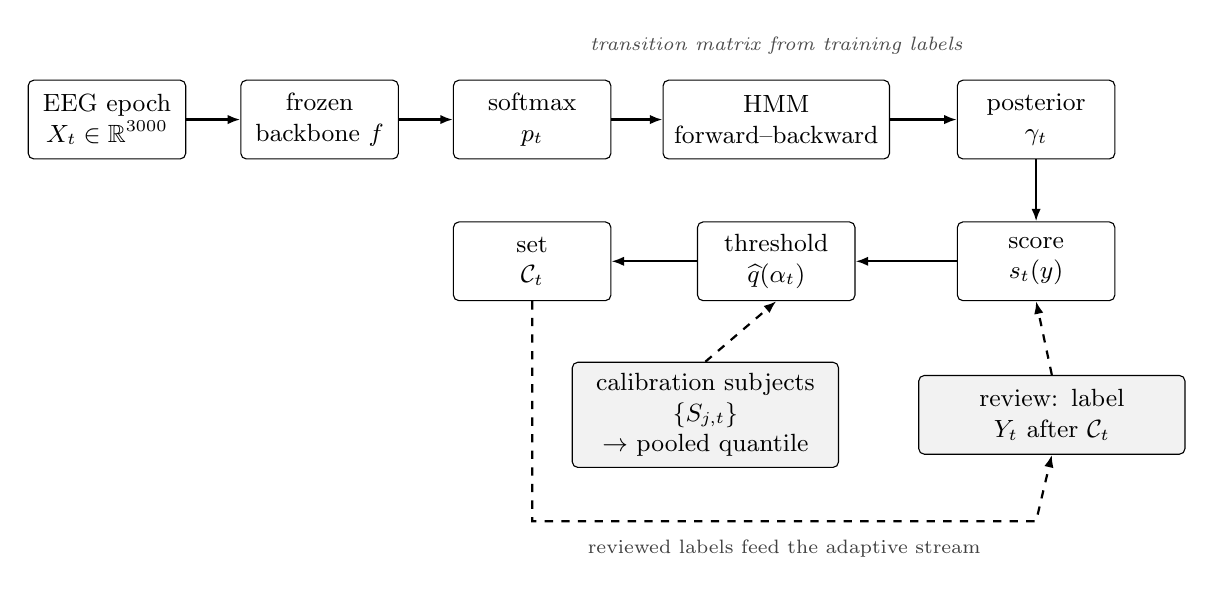
\begin{tikzpicture}[
    box/.style={draw, rounded corners=2pt, align=center,
                minimum height=10mm, minimum width=20mm,
                inner sep=4pt, font=\small},
    cal/.style={box, fill=black!5, text width=31mm},
    arr/.style={-{Latex[length=1.6mm]}, thick},
    lab/.style={font=\scriptsize\itshape, text=black!70},
    note/.style={font=\scriptsize, align=center, text=black!75}]

    % First pass: one EEG epoch becomes a temporally smoothed posterior.
    \node[box] (x) at (0,0) {EEG epoch\\$X_t\in\bR^{3000}$};
    \node[box] (f) at (2.7,0) {frozen\\backbone $f$};
    \node[box] (p) at (5.4,0) {softmax\\$p_t$};
    \node[box] (h) at (8.5,0) {HMM\\forward--backward};
    \node[box] (g) at (11.8,0) {posterior\\$\gamma_t$};

    % Second pass: posterior, calibrated threshold, and prediction set.
    \node[box] (s) at (11.8,-1.8) {score\\$s_t(y)$};
    \node[box] (q) at (8.5,-1.8) {threshold\\$\wh q(\alpha_t)$};
    \node[box] (c) at (5.4,-1.8) {set\\$\cC_t$};

    % The two auxiliary inputs sit on their own rows and cannot overlap.
    \node[cal] (cal) at (7.6,-3.75)
      {calibration subjects\\$\{S_{j,t}\}$\\$\rightarrow$ pooled quantile};
    \node[cal] (fb) at (12.0,-3.75)
      {review: label\\$Y_t$ after $\cC_t$};

    \draw[arr] (x) -- (f);
    \draw[arr] (f) -- (p);
    \draw[arr] (p) -- (h);
    \draw[arr] (h) -- (g);
    \draw[arr] (g) -- (s);
    \draw[arr] (s) -- (q);
    \draw[arr] (q) -- (c);
    \draw[arr, dashed] (cal.north) -- (q.south);
    \draw[arr, dashed] (fb.north) -- (s.south);

    % Feedback takes a separate lower route, leaving the calibration box clear.
    \draw[arr, dashed] (c.south) -- (5.4,-5.1) -- (11.8,-5.1) -- (fb.south);
    \node[note] at (8.6,-5.45) {reviewed labels feed the adaptive stream};

    \node[lab, above=2mm of h] {transition matrix from training labels};
  \end{tikzpicture}}%
  \caption{Overview of the set-valued sleep-staging pipeline. A frozen
  backbone produces epoch probabilities; forward--backward inference uses
  transition probabilities estimated from training labels to form a smoothed
  posterior. The calibration subjects determine the threshold, and the
  reviewed stage label can update the per-patient adaptive threshold. Dashed
  paths are used only in the adaptive regime.}
  \label{fig:pipeline}
\end{figure}

\subsection{Data}
\label{sec:data}

\paragraph{Sleep-EDF}
We use the Sleep-EDF Expanded corpus from PhysioNet
\citep{kemp2000,goldberger2000}, single-channel Fpz--Cz EEG at
\SI{100}{\hertz}. Two cohorts are used. \emph{Sleep-EDF-20} is the
20-subject cohort (SC400--SC419) commonly used in the sleep-staging
literature: 39 recordings, \num{42368} epochs after cropping, of which
\num{42307} carry a stage label (the remaining epochs sit inside the cropped
window but fall between scored annotations). The
\emph{extended cohort} adds the remaining cassette recordings (SC400--SC482),
giving 78 subjects and 153 recordings, and is used for the
statistical-power analysis in \Cref{sec:results-cohort}.

\paragraph{Telemetry cohort}
Sleep-EDF also contains a telemetry subset (ST700--ST721, 22 subjects,
44 recordings) recorded with different hardware on a different patient
group. It is never used for training or calibration in the cross-cohort
experiment, so it provides a genuine hardware-and-population shift rather
than a resampling of the same distribution.

\paragraph{Preprocessing}
Each recording is band-pass filtered to \SIrange{0.5}{30}{\hertz}, segmented
into \SI{30}{\second} epochs, and $z$-scored per recording. A label is
assigned to an epoch when at least 50\% of it overlaps a scored annotation.
R\&K stage~4 is merged into N3 following the AASM rule
\citep{berry2012manual}, because keeping it as a separate class would create a
sixth category with a handful of epochs and no modern counterpart.

Each recording is cropped to the scored sleep period plus 30 minutes of wake
on either side. Keeping every annotated epoch instead yields a cohort of over
\num{112000} epochs that is $65\%$ wake, which matches no published
result and distorts the class priors; the crop reproduces the canonical
Sleep-EDF-20 cohort with priors W $19.6\%$, N1 $6.6\%$, N2
$42.1\%$, N3 $13.5\%$ and REM $18.2\%$. The crop is applied
identically to every cohort and is part of the released code. Subject-wise
folds, training, and the evaluation metrics are described in
\Cref{sec:setup}.

\subsection{Notation and problem setting}
\label{sec:notation}

Let $i$ index subjects, $r$ recordings and $t$ epochs. A subject is one
patient (one or two recordings), and we use the two words interchangeably.
Each epoch has an input
$X_t\in\bR^{3000}$ (30\,s of a single EEG channel at \SI{100}{\hertz}) and a
label $Y_t\in\cY=\{W,N1,N2,N3,REM\}$ with $|\cY|=5$. A backbone $f$, trained
on subjects disjoint from the test subject, outputs
$p_t=\operatorname{softmax}(f(X_t))\in\Delta^{4}$, where $\Delta^4$ is the
probability simplex. We are given labelled calibration data from subjects
disjoint from the test subject, and we must output a set
$\cC_t\subseteq\cY$ such that
\begin{equation}
\bP\big(Y_t\in\cC_t\big)\ \ge\ 1-\alpha
\label{eq:coverage}
\end{equation}
at a nominal level $\alpha$, while keeping $|\cC_t|$ small, because every
epoch with $|\cC_t|>1$ is an epoch a human has to look at.

Two remarks fix what \Cref{eq:coverage} does and does not say. First, the
probability is over the draw of calibration and test data, not over
subjects: it is a \emph{marginal} statement, and a predictor can satisfy it
while failing on a subset of patients. Second, in sleep staging the
natural exchangeable unit is arguably the patient rather than the epoch,
and the two differ exactly in the regime of interest, where patients are
heterogeneous.

We report, alongside coverage, the \emph{set size} $|\cC_t|$, the
\emph{singleton rate} $\bP(|\cC_t|=1)$, the \emph{review workload}
$\bP(|\cC_t|>1)$, the fraction of epochs with more than one admissible stage,
the \emph{empty rate} $\bP(|\cC_t|=0)$, which also returns an epoch to the
reviewer and which the workload does not count, and a \emph{temporal
consistency} statistic, the mean Jaccard
overlap of the sets at adjacent epochs,
\begin{equation}
\mathrm{TC}=\frac{1}{|\mathcal{P}|}\sum_{(t,t+1)\in\mathcal{P}}
\frac{|\cC_t\cap\cC_{t+1}|}{|\cC_t\cup\cC_{t+1}|},
\end{equation}
where $\mathcal{P}$ contains adjacent pairs inside a recording, so that
recording boundaries are never counted. $\mathrm{TC}=1$ when neighbouring
sets are identical and $0$ when they are disjoint.

\subsection{Split conformal prediction}
\label{sec:split-cp}

Given a nonconformity score $s(x,y)$ for which smaller values indicate better
agreement between input $x$ and candidate label $y$, split CP computes
$S_j=s(X_j,Y_j)$ on $n$ calibration epochs and takes the
$\lceil(n+1)(1-\alpha)\rceil/n$ empirical quantile,
\begin{equation}
\wh q=\operatorname{Quantile}_{\lceil(n+1)(1-\alpha)\rceil/n}\big(S_1,\dots,S_n\big),
\qquad
\cC(x)=\{y\in\cY:\ s(x,y)\le\wh q\}.
\label{eq:split-cp}
\end{equation}
If the calibration and test epochs are exchangeable, then
$\bP(Y\in\cC(X))\ge 1-\alpha$ and $\bP(Y\in\cC(X))\le 1-\alpha+1/(n+1)$: the
guarantee is finite-sample and distribution-free, and both bounds are tight
for the class of all distributions \citep{vovk2005,lei2018}.

\subsection{Nonconformity scores}
\label{sec:scores}

The \emph{adaptive prediction set} score \citep{romano2020} is
\begin{equation}
s_{\aps}(x,y)=\sum_{y'\in\cY}p_{y'}(x)\,\ones\{p_{y'}(x)\ge p_y(x)\},
\label{eq:aps}
\end{equation}
the cumulative probability mass of all classes at least as likely as $y$, so
that $s_{\aps}\in[0,1]$ and smaller is better. Its set is the smallest
collection of most-likely classes whose total mass reaches $\wh q$. RAPS
\citep{angelopoulos2021raps} adds a rank penalty $\lambda_{\mathrm{reg}}\max(0,\mathrm{rank}(y)-k_{\mathrm{reg}})$
to discourage a long tail of unlikely labels.

APS is heavy-tailed near one whenever the model is badly wrong, which forces
the calibration quantile up and inflates every set. For the temporal
component we therefore use the \emph{posterior deficit}
\begin{equation}
s_{\mathrm{def}}(x,y)=\max_{k\in\cY}\gamma_x(k)-\gamma_x(y),
\label{eq:deficit}
\end{equation}
where $\gamma_x$ is a smoothed posterior (\Cref{sec:method-smoothing}). This
score is bounded in $[0,1]$, is zero exactly at the maximum-posterior stage,
and measures how far a candidate is from the posterior's mode.

A \emph{class-conditional} (Mondrian) construction \citep{vovk2012} replaces
the pooled quantile by one quantile per stage,
\begin{equation}
\wh q_y=\operatorname{Quantile}_{\lceil(n_y+1)(1-\alpha)\rceil/n_y}
\big(\{S_j:\ Y_j=y\}\big),
\label{eq:mondrian}
\end{equation}
where $n_y$ is the number of calibration epochs of stage $y$, and sets
$\cC(x)=\{y\in\cY: s(x,y)\le\wh q_y\}$. The guarantee then holds within each
stage, $\bP(Y\in\cC(X)\mid Y=y)\ge 1-\alpha$, at the price of a smaller
calibration set per class; it is the baseline we use whenever a comparison
needs stage-level coverage rather than set size.

\subsection{Adaptive conformal inference}
\label{sec:aci}

When exchangeability fails, adaptive conformal inference \citep{gibbs2021}
updates the target miscoverage after each observed label,
\begin{equation}
\alpha_{t+1}=\alpha_t+\gamma_t\big(\alpha-\ones\{Y_t\notin\cC_t\}\big),
\qquad
\cC_t=\{y:\ s(X_t,y)\le \wh q(\alpha_t)\},
\label{eq:aci}
\end{equation}
where $\wh q(\alpha_t)$ is the calibration quantile at level $1-\alpha_t$.
Along an arbitrary stream, a bounded step keeps the long-run miscoverage
within a term governed by the step size rather than letting it drift with the
shift; \citet{angelopoulos2024} show that a decaying schedule with
$\sum_t\gamma_t=\infty$ and $\sum_t\gamma_t^2<\infty$ makes that term vanish,
which is the strongest form of the guarantee and the one the corollary below
assumes.

\subsection{Temporal smoothing}
\label{sec:method-smoothing}

Sleep stages are strongly autocorrelated: an epoch of N3 is far more likely
to be followed by N3 than by W, and a per-epoch softmax discards that
information. We fit a first-order hidden Markov model to the training labels,
with transition matrix $A$ (Laplace-smoothed) and initial distribution $\pi$,
and run the forward--backward recursions in log space \emph{within each
recording} to obtain
\begin{equation}
\begin{aligned}
\gamma_t(k)&=\frac{a_t(k)b_t(k)}{\sum_{k'\in\cY}a_t(k')b_t(k')},\\
a_1(k)&=\pi_k\,p_1(k),\qquad
a_t(k)=p_t(k)\sum_{j}a_{t-1}(j)A_{jk}\quad(t\ge2),
\end{aligned}
\label{eq:forward-backward}
\end{equation}
and $b_T(k)=1$,
$b_t(k)=\sum_{j}A_{kj}\,p_{t+1}(j)\,b_{t+1}(j)$. (The forward and backward messages are
written $a$ and $b$ so that $\alpha$ and $\beta$ keep their meanings elsewhere
in the paper: the nominal level and its running ACI target, and the block
transition weight.) The recursion is $O(LK^2)$ per recording.

The smoothing uses no test labels and no test-time adaptation: it is a
deterministic transformation of the model's own output. If calibration and
test epochs are exchangeable under the score $s(\cdot,\cdot)$, they remain
exchangeable under $s(\gamma(\cdot),\cdot)$, so split CP stays valid and the
change is one of \emph{efficiency}, not of validity. That argument is the
reason we prefer smoothing to a post-hoc repair of the sets, which would
break the exchangeability argument it relies on.

\subsection{Pooled calibration and its failure mode}
\label{sec:method-pooled}

Pooled calibration guarantees that $1-\alpha$ of \emph{all} epochs are
covered, not that $1-\alpha$ of a given patient's epochs are. With $C$ the
set of calibration subjects and $S_{j,t}$ the score of epoch $t$ of subject
$j$,
\begin{equation}
\wh q_g=\operatorname{Quantile}_{\lceil(n_C+1)(1-\alpha)\rceil/n_C}
\big(\{S_{j,t}\}_{j\in C}\big),
\label{eq:global-q}
\end{equation}
which is \Cref{eq:split-cp} applied to the pooled scores. \Cref{sec:results-patient}
quantifies how far per-patient coverage departs from nominal under this rule.

\subsection{Subject-adaptive calibration with a warm-up}
\label{sec:method-sacp}

If a new subject supplies $m$ labelled epochs before deployment, those epochs
define a local threshold $\wh q_i$ by the same rule, and we deploy
\begin{equation}
\wh q_i(\lambda)=(1-\lambda)\wh q_g+\lambda\wh q_i,
\qquad \lambda\in[0,1].
\label{eq:shrunk-q}
\end{equation}
The shrinkage matters because a warm-up is short: with $m\approx 1/\alpha$
the local threshold is an extreme order statistic and its sampling variance
is large, so $\lambda=1$ trades a bias reduction for a variance increase.

\begin{proposition}[Shrinkage trade-off]
\label{prop:shrinkage}
Let subject $i$ have score CDF $F_i$ that is $\ell$-Lipschitz in a neighbourhood
of its $(1-\alpha)$-quantile $q_i^\star$, let $\Delta=q_i^\star-q_g^\star$ be
the subject's offset from the cohort quantile, and suppose $\wh q_i$ and
$\wh q_g$ are approximately unbiased with variances $\sigma^2/m$ and
$\sigma^2/n_C$. Then for a threshold $\wh q_i(\lambda)$ as in
\Cref{eq:shrunk-q}, the squared coverage gap satisfies
\begin{equation}
\bE\Big[\big(F_i(\wh q_i(\lambda))-(1-\alpha)\big)^2\Big]
\ \le\ \ell^2\Big[(1-\lambda)^2\Delta^2+\lambda^2\frac{\sigma^2}{m}
 +(1-\lambda)^2\frac{\sigma^2}{n_C}\Big],
\label{eq:shrink-bound}
\end{equation}
whose minimiser over $\lambda$ is
\begin{equation}
\lambda^\star=\frac{\Delta^2+\sigma^2/n_C}{\Delta^2+\sigma^2/n_C+\sigma^2/m}.
\label{eq:lambda-star}
\end{equation}
\end{proposition}

\begin{proof}[Proof sketch]
Write $F_i(\wh q_i(\lambda))-(1-\alpha)=F_i(\wh q_i(\lambda))-F_i(q_i^\star)$,
which is bounded in absolute value by $L|\wh q_i(\lambda)-q_i^\star|$ by the
Lipschitz condition. Expanding $\wh q_i(\lambda)-q_i^\star
=(1-\lambda)(\wh q_g-q_g^\star-\Delta)+\lambda(\wh q_i-q_i^\star)$ and taking
expectations of squares under independence of the two estimates gives
\Cref{eq:shrink-bound}; differentiating with respect to $\lambda$ and setting
the derivative to zero gives \Cref{eq:lambda-star}.
\end{proof}

Proposition~\ref{prop:shrinkage} is not a plug-in estimator: $L$, $\sigma$ and
$\Delta$ are unknown at deployment, and the Gaussian approximation to quantile
estimates is asymptotic in $m$. We use it for what it does predict --- that
$\lambda^\star\to0$ as $m\to0$, that $\lambda^\star\to1$ as $m\to\infty$, and
that adaptation pays only when the subject's offset dominates the calibration
noise, $\Delta^2\gg\sigma^2/n_C$ --- and we select $\lambda$ by leave-one-subject-out
simulation on the calibration subjects, scoring each candidate by the
one-sided mean shortfall
\begin{equation}
\mathcal{L}(\lambda)=\bE\big[\max\{0,(1-\alpha)-\widehat{\mathrm{cov}}\}\big],
\label{eq:shortfall}
\end{equation}
so that over-coverage is not rewarded; it is paid for in set size and is not
banked as a gain. Test subjects never enter this selection, which differs
from the usual practice of reporting the best $\lambda$ on test data.

\paragraph{Label-free variant}
When no warm-up labels exist, each subject is described by unlabelled
statistics $z_i=(\bar p_i,\ \overline{\max_k p_{i,k}},\ \bar H(p_i))\in\bR^{7}$
--- the mean predicted class distribution, the mean confidence and the mean
predictive entropy, with the distribution contributing five coordinates ---
and the $k$ nearest calibration subjects in this space supply a local
threshold, shrunk toward the global one with the same $\lambda$. This is an
approximation and we report it as such: it cannot be valid in general, only
when the descriptor correlates with the subject's score distribution.

\subsection{Per-patient adaptive conformal inference}
\label{sec:method-aci}

The warm-up regime presumes labelled epochs from the new patient before
deployment. In a review workflow the opposite is true: labels arrive
\emph{after} each prediction, because a technologist reviews the automatic
hypnogram. This is the feedback pattern ACI was designed for.

Running a single ACI stream over all epochs of all patients gives a pooled
guarantee once more: a hard patient can be under-covered while an easy one is
over-covered and the stream still converges. We therefore run one
\emph{independent} stream per patient $p$,
\begin{equation}
\alpha_{p,t+1}=\alpha_{p,t}+\gamma_{p,t}\big(\alpha-\ones\{Y_{p,t}\notin\cC_{p,t}\}\big),
\qquad
\cC_{p,t}=\{y:\ s_{p,t}(y)\le\wh q(\alpha_{p,t})\},
\label{eq:aci-patient}
\end{equation}
each starting at $\alpha_{p,1}=\alpha$ and each reading its threshold from the
same pooled calibration scores, so that no patient-specific calibration data
is required. The step schedule is
\begin{equation}
\gamma_{p,t}=\gamma_0/\sqrt{t+2},
\label{eq:step}
\end{equation}
which decays fast enough to stop a single misclassified stretch from
permanently loosening the threshold, and slowly enough to keep adapting over a
night. The schedule has $\sum_t\gamma_t=\infty$ but also
$\sum_t\gamma_t^2=\infty$, so it violates the square-summability condition
under which \citet{angelopoulos2024} establish their guarantee; we make
\emph{no} long-run guarantee for it, and report
the realised per-patient coverage and state in \Cref{sec:results-patient}
whether it is above or below nominal. What the procedure buys, and what we
measure, is the reallocation of coverage from easy to hard patients.

The point of running one stream per patient is that it turns ACI's pooled
long-run statement into a per-patient one. We state that implication
explicitly, because it is the only part of the construction that carries a
guarantee.

\begin{corollary}[Per-patient long-run coverage]
\label{cor:per-patient}
Suppose the threshold map $\wh q(\alpha)$ is the fixed quantile of the pooled
calibration scores, so that \Cref{eq:aci-patient} defines every set, and let
the step schedule satisfy $\gamma_t\to0$, $\gamma_t\le1$,
$\sum_t\gamma_t=\infty$ and $\sum_t\gamma_t^2<\infty$. Then for every patient
$p$ the realised miscoverage rate on that patient's stream converges to
$\alpha$,
\begin{equation}
\frac{1}{T}\sum_{t=1}^{T}\ones\{Y_{p,t}\notin\cC_{p,t}\}
\;\longrightarrow\;\alpha
\qquad (T\to\infty),
\label{eq:aci-per-patient}
\end{equation}
for an arbitrary sequence of inputs and labels, with no exchangeability
assumption within the patient.
\end{corollary}

\begin{proof}
The update \Cref{eq:aci-patient} of stream $p$ depends only on that stream's
own outcomes and on a threshold map fixed by the calibration set, so the
stream is an instance of the single-stream recursion of
\citet{angelopoulos2024}. Their long-run bound, applied stream by stream,
gives \Cref{eq:aci-per-patient}. The step \Cref{eq:step} used in the
experiments does not satisfy the summability hypothesis and therefore carries
no claim; \Cref{sec:results-aci} repeats the experiment with a schedule that
does.
\end{proof}

The scale $\gamma_0$ is a hyperparameter. We choose it by leave-one-subject-out
simulation within the calibration cohort: each calibration subject in turn
forms a stream, the remaining calibration subjects supply the score pool, and
the $\gamma_0$ that minimises the one-sided mean shortfall
\Cref{eq:shortfall} across those held-out streams --- ties broken by smaller
mean set size --- is applied unchanged to every test patient. The test cohort
never influences the choice.

\subsection{Sequence-level constructors}
\label{sec:method-seq}

A per-epoch set is free to be inconsistent with its neighbours: epoch $t$ may
admit $\{W,N1\}$ while $t+1$ admits $\{N3\}$, a transition the training labels
essentially forbid. We derived two constructors that repair this by scoring
labels in the context of the best \emph{sequence} through them, and we report
both with their properties because one of them is a useful ablation and the
other is a negative result.

\paragraph{SeqCP-Margin}
For a block of $L$ consecutive epochs inside one recording, transition cost
$\tau(a,b)=1-A_{ab}$, and weight $\beta\ge0$, define
\begin{equation}
\begin{aligned}
M_t(y)&=\min_{y_{1:L}:\,y_t=y}
\Big[\frac1L\sum_{u=1}^{L}\big(1-\gamma_u(y_u)\big)
+\frac{\beta}{L-1}\sum_{u=2}^{L}\tau(y_{u-1},y_u)\Big],\\
M^\star&=\min_{t,y}M_t(y).
\end{aligned}
\label{eq:margin}
\end{equation}
Forward and backward recursions compute every $M_t(y)$ in $O(LK^2)$; a
brute-force check over all $K^L$ paths for small blocks is part of the test
suite. We take $m_t=M_t(Y_t)-M^\star$ as the nonconformity of the true label,
calibrate $\wh\delta$ as its split-conformal quantile on calibration blocks,
and predict $\cC_t=\{y:M_t(y)-M^\star\le\wh\delta\}$. Since
$Y_t\in\cC_t\iff m_t\le\wh\delta$, this is split CP on the scalar $m_t$ and
inherits its marginal guarantee.

\begin{proposition}[Reduction at $\beta=0$]
\label{prop:reduction}
With $\beta=0$ the dynamic program factorises: for every $t$ and $y$,
\begin{equation}
M_t(y)-M^\star=\frac{1}{L}\Big(s_t(y)-\min_{k\in\cY}s_t(k)\Big),
\qquad s_t(k)=1-\gamma_t(k),
\label{eq:reduction}
\end{equation}
independently of the block. Hence SeqCP-Margin at $\beta=0$ is exactly
per-epoch split CP on the deficit score \Cref{eq:deficit}, and any difference
between the two at $\beta>0$ is attributable to the transition term alone.
\end{proposition}

\begin{proof}
At $\beta=0$ the objective separates over positions. The minimum total cost of
a path constrained to $y_t=y$ is $s_t(y)+\sum_{u\ne t}\min_k s_u(k)$, so
$M_t(y)-M^\star=\frac1L(s_t(y)-\min_k s_t(k))$ after subtracting the
unconstrained minimum $\frac1L\sum_u\min_k s_u(k)$.
\end{proof}

\begin{proposition}[Monotonicity of the centring]
\label{prop:monotone}
Let $M_t^{\mathrm{pos}}(y)=M_t(y)-\min_k M_t(k)$. Then
$M_t^{\mathrm{pos}}(y)\le M_t(y)-M^\star$ for every $t,y$, so the
position-centred sets are pointwise no larger than the globally centred ones.
\end{proposition}

\begin{proof}
$\min_k M_t(k)\ge\min_{u,k}M_u(k)=M^\star$.
\end{proof}

In practice the two coincide, because the block-optimal path on a sleep block
is usually constant and therefore visits every epoch, in which case
$\min_k M_t(k)=M^\star$ for all $t$. We keep both and report that they agree
rather than asserting a difference.

\paragraph{SeqCP-Block}
Projecting a \emph{sequence-level} conformal set onto each position gives a
simultaneous guarantee with no union bound. Calibrate the block score
\begin{equation}
S(y_{1:L})=\frac1L\sum_{t=1}^{L}\aps_t(y_t)
+\frac{\beta}{L-1}\sum_{t=2}^{L}\tau(y_{t-1},y_t)
\label{eq:block-score}
\end{equation}
on complete calibration blocks, obtaining $\wh q$, and predict
$\cC_t=\{y:M_t(y)\le\wh q\}$ with $M_t$ computed from the APS score matrix.

\begin{theorem}[Simultaneous coverage of the projection]
\label{thm:projection}
Let $\wh q$ be the split-conformal quantile of \Cref{eq:block-score} over
$n_B$ exchangeable calibration blocks. Then with probability at least
$1-\alpha$, the true block is in the block-level set, and in that
event $Y_t\in\cC_t$ for every $t=1,\dots,L$.
\end{theorem}

\begin{proof}
By \Cref{eq:split-cp}, $\bP(S(Y_{1:L})\le\wh q)\ge 1-\alpha$. If the true
block is in the block-level set then the path $y_{1:L}=Y_{1:L}$ is feasible,
so $M_t(Y_t)\le S(Y_{1:L})\le\wh q$ by the definition of $M_t$ as a minimum
over paths. Hence $Y_t\in\cC_t$ for all $t$ simultaneously.
\end{proof}

\Cref{thm:projection} is the guarantee we can prove, and
\Cref{sec:results-temporal} reports what it costs. The projection of a union
of sequences contains every label that \emph{any} admissible sequence assigns
to $t$, so it is inherently loose, and because the transition terms are
non-negative penalties the block set prefers low-transition sequences. At
$\beta\ge0.5$ the penalised block set admits a constant sequence for every
label, the projection becomes the whole label set, and the guarantee is
satisfied trivially. Even at $\beta=0$ the block mean lets one well-scored
neighbour absorb a badly scored epoch. We report this as a property of the
construction rather than of our implementation.

\subsection{What we do not claim}
\label{sec:method-claims}

The nonconformity scores are calibrated, not the model: a set can cover the
truth and still be clinically useless if it is always $\{N1,N2\}$, which is
why set size, singleton rate and review workload are reported alongside
coverage. We make no subject-conditional finite-sample guarantee under
arbitrary shift, no claim that SeqCP-Block is efficient, and no clinical
safety claim. The assumptions each result needs are stated where the result
is used.

\section{Experimental protocol}
\label{sec:setup}

\subsection{Splits}
\label{sec:splits}

\paragraph{Subject-wise folds}
Subjects are shuffled once and partitioned into five blocks. Fold $f$ tests
on block $f$, calibrates on four subjects drawn from the remaining blocks
(rotated across folds), and trains on the rest. The test blocks partition the
cohort, so every subject contributes exactly one test set across the five
folds, and no test epoch shares a subject with any calibration or training
epoch of the same fold. Per-subject statistics are computed by merging the
five folds and then averaging each subject's coverage over the seeds and
backbones that re-run that partition. Each subject therefore contributes
exactly one coverage value to the worst-patient and dispersion statistics,
and the spread we report for them is the run-to-run spread of the training,
not a spread over overlapping fold summaries.

The four-subject calibration cohort is deliberate: it is the regime a
hospital faces when it has a handful of scored nights, and it is where the
marginal guarantee is weakest. \Cref{sec:results-cohort-size} varies the size
explicitly.

\paragraph{Random-epoch split}
As a diagnostic we also train and calibrate with a 60/20/20 epoch-level
random split. Calibration and test epochs then come from the same subjects,
which is the protocol under which most published epoch-level numbers are
computed. It is not a valid estimate of deployment performance, and we use it
only to show how much of the coverage gap it hides.

\paragraph{Cross-cohort}
For the shift experiment, models are trained and calibrated on SC subjects
and tested on ST subjects, and vice versa, with no subject overlap in either
direction.

\subsection{Models and training}
\label{sec:models}

Two backbones are used throughout so that conclusions are not tied to a
single architecture: \texttt{eegnet}, a depthwise-separable convolutional
network in the style of \citet{lawhern2018} with \num{1445} parameters, and
\texttt{sleepcnn}, a four-block one-dimensional VGG-style network with global
average pooling and \num{224069} parameters. Both take a
$3000$-sample epoch and output a five-way softmax.

Training uses AdamW (learning rate $10^{-3}$, weight decay $10^{-4}$), a
cosine schedule, batch size 128, at most 40 epochs, and early stopping on a
held-out subset of the training subjects. The loss is plain cross-entropy
without class weights in every run reported here. Class weighting trades N1
recall against the calibration of the output distribution, which is exactly
the quantity CP consumes, and mixing the two settings across tables would
make coverage numbers incomparable; we therefore fix one setting and record
it in each run's metadata.

In the main matrix every configuration is run with three seeds (0, 1, 2) and
five folds, giving $15$ runs per backbone and $30$ in total; the extended
cohort and the cross-cohort experiment use seed 0 only, so their numbers are
single-seed estimates over five folds and two backbones, and the spread
reported there is across those ten runs rather than across seeds. The
run-to-run spread over seeds and backbones is
reported as the uncertainty on every headline number of the main matrix, and
per-subject statistics average a subject's coverage over those runs before
any worst-patient or dispersion statistic is formed.

\paragraph{Hardware and software}
All experiments run on a single NVIDIA RTX 4060 Laptop GPU with PyTorch;
preprocessing, conformal procedures and dynamic programs are NumPy and run on
one CPU core. Training is seeded and cuDNN is pinned to deterministic kernels,
so repeating a training run reproduces its test probabilities exactly; we
verified this by retraining one fold while the rest of the matrix occupied the
GPU and comparing the arrays. The released code reproduces every table and
figure from the raw archives with the commands recorded in the repository
README.

\subsection{Conformal procedures and hyperparameters}
\label{sec:conformal-setup}

Unless stated otherwise $\alpha=0.1$. All thresholds are computed on
calibration subjects only. The procedures compared are:

\begin{itemize}
\item \emph{Pooled APS} and \emph{pooled RAPS} on the raw softmax, with the
      split-conformal threshold \Cref{eq:split-cp}.
\item \emph{Smoothed APS}: APS on the forward--backward posterior
      \Cref{eq:forward-backward}.
\item \emph{Smoothed deficit}: the score \Cref{eq:deficit} on the same
      posterior.
\item \emph{Per-stage thresholds}: the Mondrian construction of
      \Cref{sec:scores}, applied to both the raw APS score and the smoothed
      deficit score, so that the stage-level comparison uses the same scores
      as the pooled one.
\item \emph{SACP}: warm-up calibration with shrinkage \Cref{eq:shrunk-q}, for
      label budgets $m\in\{0,10,20,40,80,160,320\}$ and $k\in\{3,5,10\}$
      neighbours for the label-free variant, with $\lambda$ chosen by
      leave-one-subject-out simulation on the calibration subjects.
\item \emph{Per-patient ACI}: one stream per patient \Cref{eq:aci-patient},
      with $\gamma_0$ chosen by leave-one-subject-out simulation from
      $\{0.005,0.01,0.02,0.05,0.1\}$.
\item \emph{SeqCP-Margin} and \emph{SeqCP-Block}: the sequence constructors of
      \Cref{sec:method-seq}, for block lengths $L\in\{10,20,30\}$ and
      transition weights $\beta\in\{0,0.5,1,2\}$.
\item \emph{Oracle}: per-subject thresholds computed on the test subject's
      own labels. Not deployable; it is the lower bound on set size at
      nominal coverage and shows how much room per-patient adaptation has.
\end{itemize}

HMM transitions are estimated from the training labels with Laplace
smoothing. Block-level comparisons restrict all methods to exactly the epochs
inside complete blocks, and the per-epoch baselines in those comparisons are
recalibrated on the same calibration epochs, so the block-length comparison
isolates the construction rather than the calibration sample.

\subsection{Metrics}
\label{sec:metrics}

Coverage is reported marginal, per stage, and per subject; from the
per-subject values we report the mean, the 10th percentile, the worst subject
and the fraction of subjects below nominal. Efficiency is reported as mean set
size, singleton rate and review workload, the fraction of epochs whose set
contains more than one stage and would therefore need adjudication. Temporal
behaviour is reported with the
Jaccard consistency statistic of \Cref{sec:notation} and with sequence
coverage, the fraction of complete blocks all of whose epochs are covered.
Classification quality is reported with accuracy, Cohen's kappa, macro-F1 and
expected calibration error (15 equal-mass bins), so that the coverage results
can be read against the underlying model quality.


\section{Results}
\label{sec:results}

All numbers are at $\alpha=0.1$ unless stated. Coverage statistics over
subjects are computed by merging per-subject coverage across the five folds
and averaging it over the seeds and backbones that re-run the same
partition, so each subject appears exactly once; the spread reported is the
run-to-run spread of the training, not a spread over patient cohorts.

\paragraph{Backbone performance}
\Cref{tab:training} reports classification quality. Both backbones sit in the
range published for Sleep-EDF on Fpz--Cz, with \texttt{sleepcnn} slightly
ahead of \texttt{eegnet} on accuracy and kappa. N1 remains the weak class for
both, and the per-stage breakdown in \Cref{tab:perclass} shows that the
marginal number hides class-level deviations in both directions. ECE is modest ($0.030$ for \texttt{eegnet}), and
\Cref{sec:results-patient} shows that this is precisely the number that fails
to detect the problem: a well-calibrated marginal predictor can still leave a
patient twelve points short of nominal coverage.

\begin{table}[t]
\centering
\small
\setlength{\tabcolsep}{4pt}
\caption{Backbone classification performance on the test subjects, over all folds and seeds (mean $\pm$ standard deviation).}
\label{tab:training}
\resizebox{\ifdim\width>\linewidth \linewidth\else\width\fi}{!}{%
\begin{tabular}{lrrrrr}
\toprule
Model & Accuracy & Cohen's $\kappa$ & Macro-F1 & ECE & Runs \\
\midrule
\texttt{eegnet} & 0.781 $\pm$ 0.042 & 0.698 $\pm$ 0.058 & 0.644 $\pm$ 0.034 & 0.030 $\pm$ 0.013 & 15 \\
\texttt{sleepcnn} & 0.803 $\pm$ 0.042 & 0.728 $\pm$ 0.058 & 0.711 $\pm$ 0.043 & 0.032 $\pm$ 0.017 & 15 \\
\bottomrule
\end{tabular}}
\end{table}


\subsection{The marginal guarantee is not the patient guarantee}
\label{sec:results-patient}

\Cref{tab:sacp} contrasts pooled calibration with the patient-level
statistics. Pooled APS reaches $0.898$ marginal coverage --- nominal to within
two thousandths --- while the worst patient is covered at $0.774$, $45\%$ of
the patients fall below $1-\alpha$, and per-patient coverage has a standard
deviation of $0.051$. The quantity that matters clinically is the
\emph{patient coverage gap},
\begin{equation}
\max_{j}\big[(1-\alpha)-\mathrm{cov}_j\big]^{+},
\end{equation}
and it is invisible in the marginal number. The first row makes the point sharper: a random-epoch split --- the
protocol under which subjects are mixed between calibration and test ---
reports $0.901$ coverage. A per-patient figure could be computed there ---
epochs carry their subject identifier --- but it would measure the epochs
shared between calibration and test rather than the subject, so the row is
reported with marginal coverage and set size only. The split that makes the
statistic estimable is the same split that makes the failure visible.

The class-conditional (Mondrian) row is the informative baseline, and it
deserves care because it is not a straw man. Conditioning the threshold on the
stage makes the mean set \emph{smaller} --- from $2.54$ to $2.29$ labels per
epoch --- because a per-class APS threshold no longer has to pay for the heavy
tail of the pooled score, and it nudges the patient statistics in the right
direction: worst-patient coverage rises from $0.774$ to $0.787$ and the
per-patient standard deviation falls from $0.051$ to $0.048$. The nudges are
small, and a paired per-patient test on the distance from nominal finds no
difference from pooled calibration (smaller for $12$ of $20$ patients,
$p=0.43$). The mechanism is that patient difficulty is strongly associated with
stage mix --- every patient is hard on N1 --- so a stage-conditional rule
equalises patients only to the extent that they differ by stage alone. What it
cannot do is adapt to a patient who is hard for reasons orthogonal to their
stage mix, and on this cohort it still leaves an $0.11$ gap at the worst
patient and $45\%$ of patients below nominal. The same limitation applies to
the per-stage threshold on the deficit score of \Cref{sec:results-score}:
conditioning reaches a patient only through their stage mix, so it reduces
the fraction of patients below nominal from $0.60$ to $0.35$ but leaves the
worst patient where it was ($0.787$ against $0.792$). That residual is the
target of \Cref{sec:results-aci}.

\begin{table}[t]
\centering
\small
\setlength{\tabcolsep}{4pt}
\caption{Coverage over patients at $\alpha=0.1$. Per-subject coverage is merged across the five subject-wise folds, so each of the 20 subjects appears exactly once. The random-epoch row is the protocol that mixes epochs from all subjects between calibration and test; a per-patient decomposition under it would measure the shared epochs rather than the subject, so the row reports marginal coverage and set size only.}
\label{tab:sacp}
\resizebox{\ifdim\width>\linewidth \linewidth\else\width\fi}{!}{%
\begin{tabular}{lrrrrrrr}
\toprule
Method & Coverage & Worst subj. & $p_{10}$ subj. & SD & Below & Set size & Singleton \\
\midrule
Random-epoch split & 0.901 & -- & -- & -- & -- & 2.542 & -- \\
Pooled (APS) & 0.898 $\pm$ 0.038 & 0.774 & 0.822 & 0.0510 & 0.45 & 2.537 $\pm$ 0.207 & 0.167 $\pm$ 0.051 \\
Pooled (RAPS) & 0.885 $\pm$ 0.037 & 0.785 & 0.836 & 0.0397 & 0.65 & 1.614 $\pm$ 0.206 & 0.472 $\pm$ 0.178 \\
Mondrian (per class) & 0.896 $\pm$ 0.031 & 0.787 & 0.835 & 0.0480 & 0.45 & 2.294 $\pm$ 0.157 & 0.230 $\pm$ 0.062 \\
$k$NN subject (APS) & 0.894 $\pm$ 0.040 & 0.759 & 0.828 & 0.0536 & 0.50 & 2.509 $\pm$ 0.214 & 0.170 $\pm$ 0.049 \\
Warm-up SACP, $m=80$ & 0.897 $\pm$ 0.036 & 0.782 & 0.820 & 0.0496 & 0.40 & 2.552 $\pm$ 0.299 & 0.172 $\pm$ 0.055 \\
Warm-up SACP, $m=320$ & 0.891 $\pm$ 0.031 & 0.769 & 0.829 & 0.0516 & 0.50 & 2.519 $\pm$ 0.151 & 0.155 $\pm$ 0.045 \\
Oracle per patient & 0.901 $\pm$ 0.000 & 0.901 & 0.901 & 0.0004 & 0.00 & 2.492 $\pm$ 0.230 & 0.180 $\pm$ 0.058 \\
Per-patient ACI (APS) & 0.904 $\pm$ 0.010 & 0.886 & 0.892 & 0.0117 & 0.50 & 2.491 $\pm$ 0.203 & 0.177 $\pm$ 0.060 \\
Per-patient ACI (deficit) & 0.898 $\pm$ 0.007 & 0.872 & 0.891 & 0.0097 & 0.70 & 1.575 $\pm$ 0.271 & 0.831 $\pm$ 0.072 \\
\bottomrule
\end{tabular}}
\par\vspace{2pt}{\footnotesize ``Coverage'' is marginal over epochs (mean $\pm$ SD over the runs); ``Worst subj.'' is the minimum per-subject coverage over the runs; ``Below'' is the fraction of subjects below $1-\alpha$; ``SD'' is the standard deviation of per-subject coverage. Each subject contributes one value per run, the runs being five folds $\times$ three seeds $\times$ two backbones; set size and singleton rate are averaged over the same runs.}
\end{table}


\subsection{Posterior smoothing is the largest efficiency lever}
\label{sec:results-score}

\Cref{tab:temporal} compares nonconformity scores on the same epochs and the
same calibration data. Replacing the raw-softmax APS score with the smoothed
posterior deficit reduces the mean set size from $2.54$ to $1.53$ labels per
epoch at essentially the same coverage ($0.898$ against $0.889$, a difference
within the run spread), and raises the Jaccard consistency statistic from
$0.68$ to $0.94$. Both sit close to nominal --- the deficit score $1.1$ points
below and APS $0.2$ points below --- and the residual gap of
the deficit score is the finite-sample fluctuation of the split-conformal
threshold --- the guarantee is in expectation over calibration draws, not a
statement about one calibration set --- and it is smaller than the
run-to-run spread. The mechanism is visible in the singleton rate, which rises
from $0.17$ to $0.84$: most epochs are predicted as a single stage, which is
the behaviour a reviewing technologist wants. The review workload --- the
fraction of epochs whose set contains more than one stage and would need
adjudication --- falls from $0.76$ to $0.16$ over the same runs. A second
asymmetry is not in the table: pooled APS returns an \emph{empty} set on
$6.8\%$ of epochs, where no stage clears the threshold, and those epochs also
go to the reviewer even though the workload definition does not count them.
The deficit score is never empty ($0.000$), because its score has an atom at
zero and the posterior mode always admits itself. Adding empty sets to the
workload leaves the comparison unchanged ($0.83$ against $0.16$).

The efficiency is not free at the class level. \Cref{tab:perclass} breaks
coverage down by stage. Pooled APS over-covers the rare and difficult stages
--- N1 at $0.96$ and REM at $0.985$ --- because the heavy tail of its score
forces a loose threshold, and it under-covers W ($0.81$) and N3 ($0.87$).
Smoothing the APS score redistributes the imbalance rather than removing it:
W falls to $0.75$ while N1 stays at $0.95$. The deficit score removes the
looseness where the model is confident and pays for
it on N1, whose coverage falls to $0.43$: when the model is confidently wrong
on an N1 epoch, the posterior deficit of the true N1 is large, so the set
omits the stage exactly where the error is.

The repair is one line of calibration rather than a different score:
thresholding the same deficit score per stage (\Cref{eq:mondrian}). Every
stage then lands between $0.899$ and $0.909$ at $1.74$ labels per epoch --- a
quarter fewer than conditioning APS on the stage ($2.29$) and almost a third
fewer than pooled APS ($2.54$). It also lowers the fraction of patients below
nominal from $0.60$ to $0.35$, although the worst patient is unchanged
($0.787$ against $0.792$ for the pooled deficit threshold). What conditioning costs is review
workload, which rises from $0.16$ to $0.49$ because the sets add a second
stage whenever the model's evidence is weak, and adjacent-set consistency,
which falls from $0.94$ to $0.88$. We therefore report the unconditioned
deficit score as the efficiency frontier and the per-stage version as the
deployment default when an omitted stage is costly; the per-patient analysis
below is marginal over stages and is unaffected.

\begin{table}[t]
\centering
\small
\setlength{\tabcolsep}{4pt}
\caption{Coverage per stage at $\alpha=0.1$, averaged over the 30 runs. Nominal coverage is 0.90 for every stage.}
\label{tab:perclass}
\resizebox{\ifdim\width>\linewidth \linewidth\else\width\fi}{!}{%
\begin{tabular}{lrrrrr}
\toprule
Stage & Pooled APS & Smoothed APS & Smoothed deficit & Deficit, per stage & Mondrian APS \\
\midrule
W & 0.812 & 0.747 & 0.925 & 0.904 & 0.887 \\
N1 & 0.961 & 0.953 & 0.432 & 0.902 & 0.904 \\
N2 & 0.899 & 0.924 & 0.933 & 0.909 & 0.897 \\
N3 & 0.865 & 0.923 & 0.912 & 0.899 & 0.899 \\
REM & 0.985 & 0.980 & 0.912 & 0.905 & 0.906 \\
\midrule
Mean $|\cC_t|$ & 2.537 & 2.223 & 1.531 & 1.741 & 2.294 \\
\bottomrule
\end{tabular}}
\par\vspace{2pt}{\footnotesize Each coverage cell is the fraction of epochs of that stage whose set contains the true stage, averaged over the runs; the averages weight the stages unequally because the test blocks differ, so the run-to-run spread is in the released JSON. The bottom row is the mean set size over all epochs, the counterpart of those coverage numbers. The last two columns threshold per stage, on the deficit score and on the raw APS score respectively, so their stage coverage is near nominal by construction.}
\end{table}


The recursion costs nothing at
inference: $O(LK^2)$ per recording, measured at
\SIrange{30}{40}{\micro\second} per epoch --- a few tens of milliseconds for
a whole recording --- on one CPU core (\texttt{scripts/benchmark\_smoothing.py}
reproduces the measurement on the machine at hand).

APS on the smoothed posterior sits between the two: smoothing alone helps
($2.54\to2.22$ labels at $0.903$ coverage, consistency $0.75$),
but the heavy tail of the APS score limits how much, and the deficit score
removes it. RAPS narrows the tail at the cost of a rank hyperparameter that
must be tuned on held-out calibration data; it reaches $1.61$ labels at
$0.885$ coverage with $47\%$ singletons, better than APS and short of the
deficit score, and we do not pursue it further because the deficit score needs
no extra hyperparameter.

The ordering does not depend on the nominal level. Recomputing both scores on
the same fitted models at $\alpha\in\{0.05,0.2\}$, the deficit score uses
fewer labels at every level ($2.16$ against $2.97$ at $\alpha=0.05$; $1.05$
against $2.00$ at $\alpha=0.2$), and at $\alpha=0.2$ it over-covers where APS
under-covers ($0.825$ against $0.794$ for a nominal $0.80$). The gap in
coverage between the two score families is therefore not an artefact of the
one level the paper reports in its tables.

\subsection{Calibration-cohort size and the label budget}
\label{sec:results-cohort-size}

\Cref{tab:cohort-size} isolates the calibration-cohort axis by subsampling
$k$ of the four calibration subjects, refitting the pooled threshold, and
repeating the subsample fifty times. Marginal coverage of the pooled APS
threshold converges quickly in $k$, but the worst of its four test subjects
--- a per-run minimum, averaged over runs, not the merged-cohort worst
patient --- plateaus around $0.84$, six points below nominal; the deficit
score's corresponding statistic is flat in $k$ ($0.848$ at $k=1$, $0.849$ at
$k=4$). The patient gap is therefore not calibration-sampling noise: it is
present with a single calibration subject and essentially unchanged with all
four. Adding calibration patients buys a less noisy estimate of the wrong
quantity.

\Cref{fig:budget} reports the label-budget regime.
Proposition~\ref{prop:shrinkage} says the optimal shrinkage weight rises with
the warm-up budget $m$; the obstacle is estimating it. Warm-up from the new
patient helps only if the shrinkage weight is chosen well, and at this cohort
size leave-one-subject-out selection cannot choose it. The criterion is
degenerate: it returns $\lambda=0$ at every budget up to $m=80$ in
$16$ of the $30$ runs, and where it does select a positive weight the choice
is unstable across folds and seeds --- at $m=80$ the same budget selects $0$,
$0.25$, $0.5$, $0.75$ and $1$ in different runs. Merging per-subject coverage
across folds, the curve does not improve and the largest budget degrades it:
worst-patient coverage is $0.774$ at $m=0$ and $0.769$ at $m=320$, with no
budget in between exceeding $0.783$.

\Cref{tab:sacp-lambda} holds the shrinkage weight fixed instead of selecting
it, and shows how much of the loss is the selection rule. Short warm-ups are
not marginal, they are catastrophic: at $m=20$ the worst patient falls from
$0.780$ under the pooled threshold to $0.685$ at $\lambda=0.5$ and $0.590$ at
$\lambda=1$. At $m=160$ the same weights leave the worst patient at $0.788$
and $0.797$ against $0.772$ for the pooled threshold --- a gain of at most two
and a half points, against the thirteen-point gap to the oracle --- and at
$m=320$ the ordering reverses ($0.766$ pooled, $0.776$ at $\lambda=0.5$,
$0.755$ at $\lambda=1$). So the degeneracy of the selection is not the whole
story: even a fixed, generous weight cannot close the patient gap at this
cohort size, and at small budgets it does much worse.

The mechanism is visible in what a warm-up actually contains. A warm-up is a
poor sample of the night it is deployed on.
At $m=160$ it covers the first $80$ minutes, in which wake accounts for
$42\%$ of epochs and REM for none, against $18\%$ and $20\%$ over the rest of
the night (reproduced by \texttt{scripts/warmup\_composition.py}), so the
threshold is estimated on one stage mix and applied to another. At $m=20$ the
estimate is also built from twenty epochs, so it carries the variance term of
\Cref{eq:shrink-bound} on top of the bias.

\begin{table}[t]
\centering
\footnotesize
\setlength{\tabcolsep}{4pt}
\caption{Warm-up calibration at fixed shrinkage weights, $\alpha=0.1$.}
\label{tab:sacp-lambda}
\resizebox{\ifdim\width>\linewidth \linewidth\else\width\fi}{!}{%
\begin{tabular}{llrrrr}
\toprule
$m$ & $\lambda$ & Coverage & Worst subj. & SD & Set size \\
\midrule
$m=20$ & 0 & 0.899 & 0.780 & 0.050 & 2.541 \\
 & 0.5 & 0.868 & 0.685 & 0.068 & 2.407 \\
 & 1 & 0.882 & 0.590 & 0.104 & 2.763 \\
\addlinespace[2pt]
$m=80$ & 0 & 0.900 & 0.780 & 0.050 & 2.538 \\
 & 0.5 & 0.884 & 0.788 & 0.049 & 2.440 \\
 & 1 & 0.893 & 0.731 & 0.066 & 2.617 \\
\addlinespace[2pt]
$m=160$ & 0 & 0.899 & 0.772 & 0.051 & 2.558 \\
 & 0.5 & 0.893 & 0.788 & 0.044 & 2.501 \\
 & 1 & 0.903 & 0.797 & 0.051 & 2.619 \\
\addlinespace[2pt]
$m=320$ & 0 & 0.899 & 0.766 & 0.054 & 2.582 \\
 & 0.5 & 0.892 & 0.776 & 0.051 & 2.513 \\
 & 1 & 0.895 & 0.755 & 0.059 & 2.574 \\
\bottomrule
\end{tabular}}
\par\vspace{2pt}{\footnotesize Within a block, the rows share the same evaluation epochs: the first $m$ epochs of each patient are used only for warm-up and are excluded from every row, so the $\lambda=0$ row is the pooled threshold applied to the post-warm-up epochs and the other rows differ from it only in the shrinkage weight. Per-subject coverage is merged across folds and averaged over seeds and backbones. Over the 30 runs, leave-one-subject-out selection returned zero for every budget up to $m=80$ in 16 of them; the full selection histogram is in the released JSON.}
\end{table}


We report this as a negative result rather than a design choice. With four
calibration subjects there is too little held-out data to separate the gain
from adapting the threshold to the new patient from the loss from estimating
it on a handful of epochs, and the selected weight appears to be decided by
which of the four subjects happens to be hardest. The label-free
$k$-nearest-subject variant fails for a structural reason: with four
calibration subjects, $k=3$ already draws on most of the pool and gives the
worst patient $0.759$, below the pooled $0.774$, while $k\ge5$ is the whole
pool and returns the pooled threshold exactly. With four subjects there is
no neighbourhood to select. Section~\ref{sec:results-aci} gives the alternative
that needs no warm-up labels at all.

\Cref{fig:pareto} puts the same sweep on the efficiency--reliability plane.
Across a factor of $32$ in label budget the warm-up path stays within a
tenth of a label and one point of worst-patient coverage of the pooled point,
and never approaches the oracle anchor, which sits at essentially the same set
size but at nominal worst-patient coverage. The shortfall is
therefore not a question of choosing a better budget: it is the distance
between what a per-patient threshold could do with the patient's own labels
and what any warm-up rule achieves.

\begin{figure}[t]
  \centering
  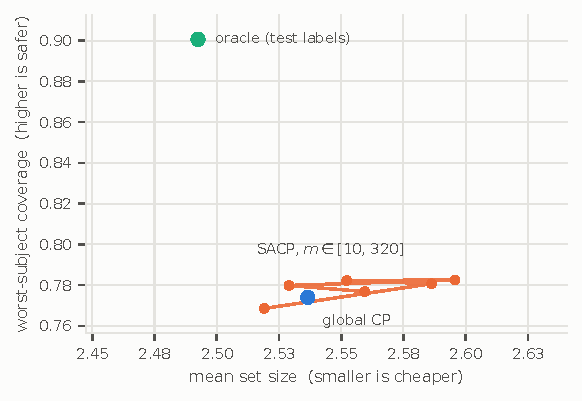
\includegraphics[width=0.72\linewidth]{fig3_pareto.pdf}
  \caption{Worst-patient coverage against mean set size along the warm-up
  budget $m\in\{10,\dots,320\}$, with the shrinkage weight selected by
  leave-one-subject-out simulation at each budget. The blue point is pooled
  calibration, which is also the $m=0$ rule, and the teal point is the oracle
  per-patient threshold computed on the test patient's own labels. The path
  stays next to the pooled point across the whole budget range, and the
  distance to the oracle is what no warm-up rule closes.}
  \label{fig:pareto}
\end{figure}

\begin{table}[t]
\centering
\footnotesize
\setlength{\tabcolsep}{4pt}
\caption{Coverage against the number of calibration subjects $k$, subsampling the available calibration subjects and repeating 50 times per run; rows are averaged over all runs, and $\pm$ is the standard deviation across runs. ``worst'' is the minimum per-subject coverage within a run (each run tests four subjects), averaged over runs, so it is not the merged-cohort worst patient of \Cref{tab:sacp}; it is the quantity that this sweep can hold fixed while $k$ varies. The deficit score's worst-patient coverage is flat in $k$: the patient gap is not calibration-sampling noise.}
\label{tab:cohort-size}
\resizebox{\ifdim\width>\linewidth \linewidth\else\width\fi}{!}{%
\begin{tabular}{rrrrr}
\toprule
\multicolumn{1}{c}{} & \multicolumn{2}{c}{APS} & \multicolumn{2}{c}{Posterior deficit} \\\cmidrule(lr){2-3}\cmidrule(lr){4-5}
$k$ & cov. & worst & cov. & worst \\
\midrule
1 & 0.882\,$\pm$\,0.037 & 0.819\,$\pm$\,0.058 & 0.887\,$\pm$\,0.042 & 0.848\,$\pm$\,0.058 \\
2 & 0.894\,$\pm$\,0.036 & 0.833\,$\pm$\,0.060 & 0.886\,$\pm$\,0.043 & 0.847\,$\pm$\,0.059 \\
3 & 0.896\,$\pm$\,0.038 & 0.837\,$\pm$\,0.062 & 0.889\,$\pm$\,0.044 & 0.850\,$\pm$\,0.060 \\
4 & 0.898\,$\pm$\,0.038 & 0.838\,$\pm$\,0.062 & 0.889\,$\pm$\,0.044 & 0.849\,$\pm$\,0.061 \\
\bottomrule
\end{tabular}}
\par\vspace{2pt}{\footnotesize APS columns are the raw-softmax score; deficit columns use the smoothed posterior deficit. Nominal coverage is 0.900. Calibration pool: 4 subjects.}
\end{table}


\begin{figure}[t]
  \centering
  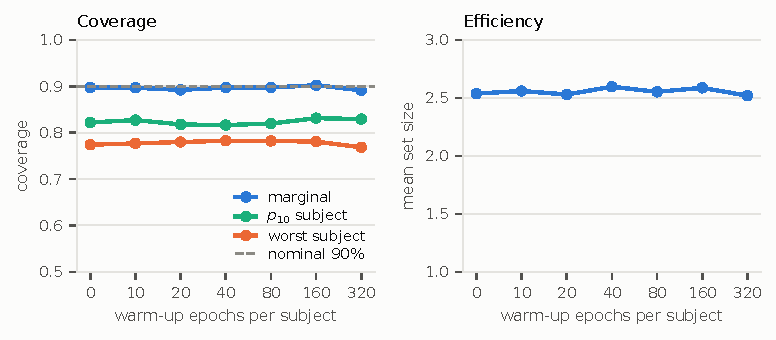
\includegraphics[width=\linewidth]{fig1_budget.pdf}
  \caption{Left: marginal, $p_{10}$ and worst-patient coverage against the
  number of labelled warm-up epochs from the new patient. Right: the
  corresponding mean prediction-set size. The horizontal line marks nominal
  coverage.}
  \label{fig:budget}
\end{figure}

\subsection{Per-patient adaptation collapses the coverage spread}
\label{sec:results-aci}

\Cref{tab:aci} is the central result. Pooled calibration leaves a spread of
$0.051$ across patients and a worst patient at $0.774$. Running one ACI
stream per patient, with the step scale chosen on held-out calibration
streams, collapses the spread to $0.012$ and lifts the worst patient to
$0.886$, at a mean set size of $2.49$ against $2.54$. The deficit score
inherits the correction: its worst patient moves from $0.792$ to $0.872$ at
essentially unchanged set size ($1.53$ to $1.58$), so the efficiency gain of
\Cref{sec:results-score} and the spread collapse of this section compose.

The comparison is paired by patient, and we test the quantity the section is
about rather than the mean. Mean per-patient coverage changes little and not
significantly ($0.896$ to $0.904$, Wilcoxon signed-rank $p=0.84$), but the
distance of a patient's coverage from nominal is smaller under ACI for
$19$ of the $20$ patients (median reduction $0.025$, $p=9.5\times10^{-6}$),
and smaller than under Mondrian for $19$ of $20$ ($p=3.8\times10^{-6}$). The
one patient who moves away from nominal is above it under both rules and
moves by six thousandths (from $0.908$ to $0.914$), well inside the
run-to-run spread. Mondrian is the nearest
alternative on this statistic, and it is not distinguishable from pooled
calibration ($12$ of $20$, $p=0.43$), which is why we read the Mondrian
changes in \Cref{sec:results-patient} as directionally right but not
significant on this cohort.

\Cref{tab:aci-sweep} reports the same experiment at each step scale rather
than at the selected one. The worst patient improves monotonically in
$\gamma_0$ for both scores, from $0.810$ to $0.888$ (APS) and from $0.828$ to
$0.882$ (deficit), and the mean absolute deviation from nominal falls from
$0.030$ to $0.006$ and from $0.026$ to $0.006$. Larger steps are not free: the
fraction of patients below nominal rises from $0.40$ to $0.75$ (APS), because
the recursion pulls every stream toward the marginal rate, and once the spread
has collapsed it is the mean, not the worst patient, that becomes the binding
quantity. The grid stops at $\gamma_0=0.1$ for that reason --- the
spread reduction has saturated while the fraction below nominal is still rising.
The LOSO-selected value ($0.062$ for APS, $0.075$ for the deficit score) sits
below the grid's best row and costs two thousandths of worst-patient coverage
for APS and one point for the deficit score, relative to the best fixed value
in hindsight; that is the price of choosing without the test cohort, and both
are small against the eleven- and eight-point gains over pooled calibration.

One property of \Cref{eq:step} deserves an explicit check. The schedule has
$\sum_t\gamma_t^2=\infty$ and therefore falls outside the
square-summability condition under which the long-run ACI bound is proved, so
the improvement above cannot be attributed to the theory. Repeating the
identical experiment with $\gamma_t=\gamma_0/(t+2)^{0.6}$, which does meet the
condition, leaves the conclusion in place and slightly weaker: worst-patient
coverage $0.877$ against $0.774$ for pooled calibration, per-patient SD
$0.015$ against $0.051$, at a mean set size of $2.51$. The faster-decaying
step adapts more slowly within a night, which is the expected
price of a guarantee that the default schedule does not carry. That guarantee
is \Cref{cor:per-patient}, and it is asymptotic: it says that each patient's
realised miscoverage converges to $\alpha$ as the stream grows, while a night
contributes only a few hundred epochs, so it predicts the direction of the
effect rather than its size. The default schedule is left in the paper
because it is what an implementation would use; the poly-schedule run is
there so that the reader can see the size of the effect under a schedule for
which the corollary actually applies.

\begin{figure}[t]
  \centering
  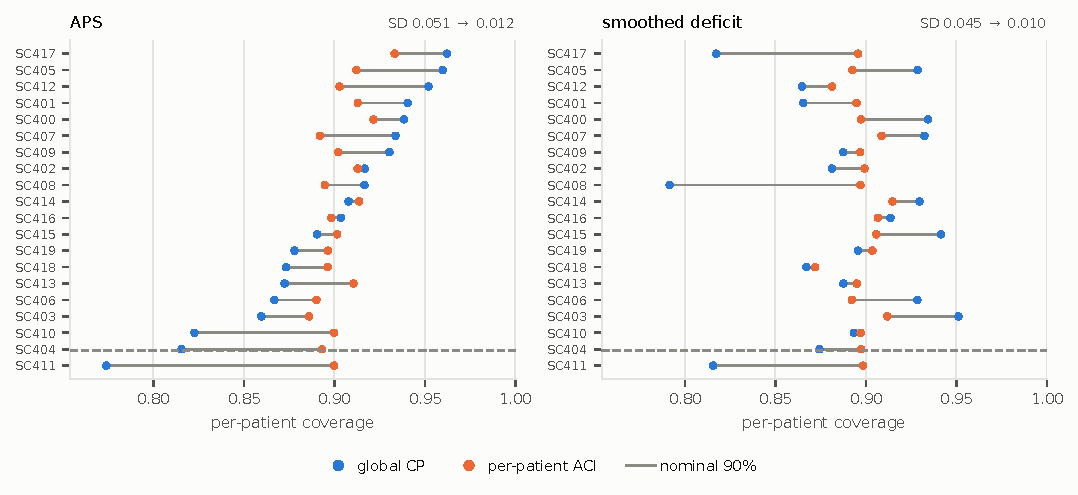
\includegraphics[width=0.9\linewidth]{fig2_subjects.pdf}
  \caption{Per-patient coverage under pooled calibration and under per-patient
  ACI, one line segment per patient, sorted by pooled coverage. Patients to
  the left of the nominal line gain coverage; patients to the right give up
  coverage they did not need.}
  \label{fig:subjects}
\end{figure}

\Cref{fig:subjects} shows the mechanism directly. The reallocation is the
point: the mean coverage is unchanged, and a fraction of patients end up a
hair below nominal by construction, so the fraction-below statistic is not
informative here --- the dispersion and the worst patient are. A single
stream over all patients cannot do this by construction: it returns one
threshold for every patient, so it can move the marginal rate but not the
per-patient dispersion, which is the reason we run one stream per patient.
We therefore do not tabulate a single-stream variant; the comparison that
matters is against the pooled threshold, which is exactly what a single
stream converges to.

\begin{table}[t]
\centering
\small
\setlength{\tabcolsep}{4pt}
\caption{Per-patient adaptive conformal inference at $\alpha=0.1$. Each patient is an independent stream; the step scale is chosen by leave-one-subject-out simulation on the calibration subjects and then applied unchanged to the test cohort.}
\label{tab:aci}
\resizebox{\ifdim\width>\linewidth \linewidth\else\width\fi}{!}{%
\begin{tabular}{lrrrrrrrr}
\toprule
Method & Cov. & Worst & SD & MAD$_\alpha$ & Below & Size & Sing. & Cons. \\
\midrule
Global CP (APS) & 0.898 $\pm$ 0.038 & 0.774 & 0.051 & 0.040 & 0.450 & 2.537 $\pm$ 0.207 & 0.167 $\pm$ 0.051 & 0.680 $\pm$ 0.037 \\
Global CP (deficit) & 0.889 $\pm$ 0.044 & 0.792 & 0.045 & 0.036 & 0.600 & 1.531 $\pm$ 0.325 & 0.841 $\pm$ 0.080 & 0.942 $\pm$ 0.018 \\
Per-patient ACI (APS) & 0.904 $\pm$ 0.010 & 0.886 & 0.012 & 0.009 & 0.500 & 2.491 $\pm$ 0.203 & 0.177 $\pm$ 0.060 & 0.675 $\pm$ 0.020 \\
Per-patient ACI (deficit) & 0.898 $\pm$ 0.007 & 0.872 & 0.010 & 0.007 & 0.700 & 1.575 $\pm$ 0.271 & 0.831 $\pm$ 0.072 & 0.940 $\pm$ 0.014 \\
\bottomrule
\end{tabular}}
\par\vspace{2pt}{\footnotesize Coverage statistics merge per-subject coverage across folds and average each subject over the runs (folds $\times$ seeds $\times$ backbones). Mean LOSO-selected $\gamma_0$ over the runs: aps $= 0.0623$, deficit $= 0.075$. Set size and consistency are averaged over the same runs.}
\end{table}

\begin{table}[t]
\centering
\small
\setlength{\tabcolsep}{4pt}
\caption{Sensitivity of per-patient ACI to the step scale $\gamma_0$ at $\alpha=0.1$. None of these rows is selected on test data; the deployable choice is the LOSO-selected one in \Cref{tab:aci}.}
\label{tab:aci-sweep}
\resizebox{\ifdim\width>\linewidth \linewidth\else\width\fi}{!}{%
\begin{tabular}{lrrrrr}
\toprule
Method & Coverage & Worst subj. & $p_{10}$ subj. & Frac.\ below & Set size \\
\midrule
Per-patient ACI (APS), $\gamma_0=0.005$ & 0.904 $\pm$ 0.026 & 0.810 & 0.864 & 0.400 & 2.566 $\pm$ 0.185 \\
Per-patient ACI (APS), $\gamma_0=0.01$ & 0.908 $\pm$ 0.018 & 0.848 & 0.872 & 0.300 & 2.581 $\pm$ 0.197 \\
Per-patient ACI (APS), $\gamma_0=0.02$ & 0.908 $\pm$ 0.011 & 0.875 & 0.887 & 0.400 & 2.553 $\pm$ 0.199 \\
Per-patient ACI (APS), $\gamma_0=0.05$ & 0.902 $\pm$ 0.006 & 0.885 & 0.891 & 0.500 & 2.469 $\pm$ 0.177 \\
Per-patient ACI (APS), $\gamma_0=0.1$ & 0.898 $\pm$ 0.004 & 0.888 & 0.890 & 0.750 & 2.409 $\pm$ 0.163 \\
Per-patient ACI (deficit), $\gamma_0=0.005$ & 0.894 $\pm$ 0.030 & 0.828 & 0.859 & 0.600 & 1.579 $\pm$ 0.255 \\
Per-patient ACI (deficit), $\gamma_0=0.01$ & 0.898 $\pm$ 0.021 & 0.859 & 0.862 & 0.600 & 1.613 $\pm$ 0.260 \\
Per-patient ACI (deficit), $\gamma_0=0.02$ & 0.900 $\pm$ 0.014 & 0.860 & 0.884 & 0.600 & 1.616 $\pm$ 0.268 \\
Per-patient ACI (deficit), $\gamma_0=0.05$ & 0.899 $\pm$ 0.007 & 0.873 & 0.887 & 0.550 & 1.590 $\pm$ 0.267 \\
Per-patient ACI (deficit), $\gamma_0=0.1$ & 0.898 $\pm$ 0.004 & 0.882 & 0.889 & 0.650 & 1.562 $\pm$ 0.265 \\
\bottomrule
\end{tabular}}
\end{table}


\subsection{Sequence constructors: a negative result}
\label{sec:results-temporal}

\Cref{tab:temporal} reports the dynamic-programming constructors alongside
their per-epoch comparators. The first block uses every test epoch and
includes the per-stage deficit threshold of \Cref{sec:results-score}, so that
the score-family comparison is in one place; the constructor blocks use only
the epochs inside complete blocks, and the per-epoch baseline immediately
above the SeqCP-Margin block is recalibrated on exactly those epochs. Three
observations follow, and they are the reason we do not present these
constructors as a contribution.

\emph{At $\beta=0$ the margin constructor is exactly per-epoch split CP} on the
deficit score (Proposition~\ref{prop:reduction}). The numerical check in the
test suite confirms the identity to machine precision, and
\Cref{tab:temporal} confirms it at the level of realised coverage and set
size: the $\beta=0$ row and the baseline above it agree to every reported
digit. This is not a nuisance: it is what allows the $\beta>0$ rows to be
interpreted as the effect of the transition term alone.

\emph{At $\beta>0$ the sets get larger.} The block-level set is a union over
admissible sequences, and the transition penalty makes low-transition
sequences cheap; at $\beta\ge0.5$ a constant sequence is admissible for every
label, the projection is the whole label set, and sequence coverage is
$1.000$ by triviality. The simultaneous guarantee of
Theorem~\ref{thm:projection} holds and is vacuous. \Cref{tab:temporal}'s
SeqCP-Block rows show this directly.

\emph{The transition structure is already in the score.} The smoothed
posterior that the deficit score is computed from has absorbed the same
Markov structure that the dynamic program is meant to exploit. Re-imposing it
at the level of the set adds looseness rather than information. This is why
the efficiency gain in \Cref{sec:results-score} comes from smoothing, not
from sequence construction, and it is the substantive lesson of the
ablation.

\Cref{fig:hypnogram} shows the consequence on a real recording: pooled APS
produces sets that flicker at transitions, the deficit score produces stable
singleton sets through stable stretches and wider sets at transitions, and
per-patient ACI widens the sets for a patient whose pooled coverage was low.

\begin{figure}[t]
  \centering
  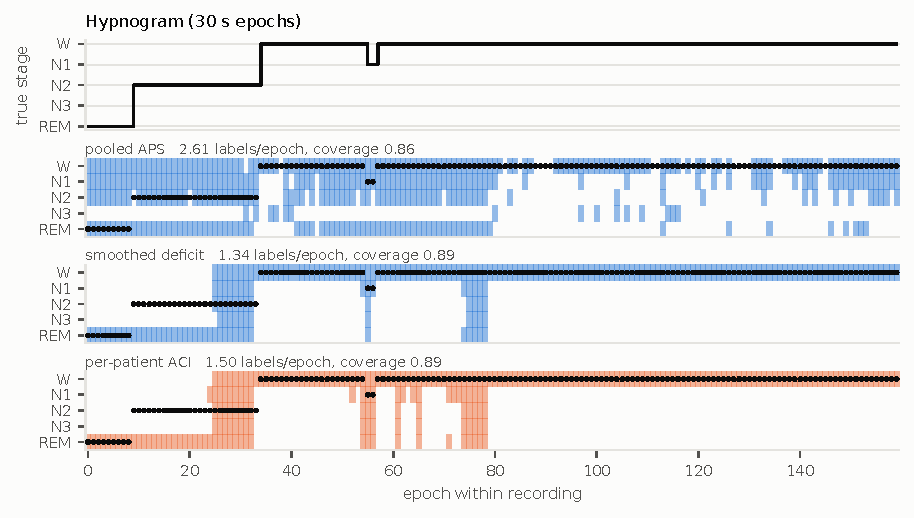
\includegraphics[width=\linewidth]{fig4_hypnogram.pdf}
  \caption{A \num{160}-epoch window of one test recording (subject SC409),
  chosen because it spans a stage transition. Top: the scored hypnogram.
  Panels: one row per stage, with a shaded cell where that stage is in the
  prediction set under pooled APS, smoothed deficit, and per-patient ACI. The
  black dots repeat the true stage inside each panel, so an epoch is covered
  exactly when its dot lies on a shaded cell; the label count and coverage
  printed with each panel are over this window only.}
  \label{fig:hypnogram}
\end{figure}

\begin{table}[t]
\centering
\small
\setlength{\tabcolsep}{4pt}
\caption{Temporal conformal prediction at $\alpha=0.1$, block length $L=10$. The first four rows use every test epoch; the rows below them use only the epochs inside complete blocks, and the per-epoch baseline above the SeqCP-Margin block is recalibrated on exactly those epochs.}
\label{tab:temporal}
\resizebox{\ifdim\width>\linewidth \linewidth\else\width\fi}{!}{%
\begin{tabular}{lrrrrrr}
\toprule
Method & Coverage & Set size & Singleton & Review & Consistency & Seq.\ coverage \\
\midrule
Smoothed deficit (all epochs) & 0.889 $\pm$ 0.044 & 1.531 $\pm$ 0.325 & 0.841 $\pm$ 0.080 & 0.159 $\pm$ 0.080 & 0.942 $\pm$ 0.018 & -- \\
Smoothed deficit, per stage & 0.903 $\pm$ 0.034 & 1.741 $\pm$ 0.252 & 0.506 $\pm$ 0.104 & 0.494 $\pm$ 0.104 & 0.884 $\pm$ 0.016 & -- \\
Smoothed APS (all epochs) & 0.903 $\pm$ 0.037 & 2.223 $\pm$ 0.170 & 0.229 $\pm$ 0.053 & 0.712 $\pm$ 0.062 & 0.753 $\pm$ 0.036 & -- \\
Per-epoch APS (all epochs) & 0.898 $\pm$ 0.038 & 2.537 $\pm$ 0.207 & 0.167 $\pm$ 0.051 & 0.765 $\pm$ 0.060 & 0.680 $\pm$ 0.037 & -- \\
\addlinespace[3pt]
Smoothed deficit, $L=10$ epochs & 0.889 $\pm$ 0.045 & 1.535 $\pm$ 0.326 & 0.840 $\pm$ 0.080 & 0.160 $\pm$ 0.080 & 0.942 $\pm$ 0.018 & -- \\
SeqCP-Margin L10, $\beta=0$ & 0.889 $\pm$ 0.045 & 1.535 $\pm$ 0.326 & 0.840 $\pm$ 0.080 & 0.160 $\pm$ 0.080 & 0.942 $\pm$ 0.018 & 0.668 $\pm$ 0.089 \\
SeqCP-Margin L10, $\beta=0.5$ & 0.890 $\pm$ 0.045 & 1.941 $\pm$ 0.616 & 0.688 $\pm$ 0.215 & 0.312 $\pm$ 0.215 & 0.865 $\pm$ 0.061 & 0.682 $\pm$ 0.096 \\
SeqCP-Margin L10, $\beta=1$ & 0.891 $\pm$ 0.045 & 1.993 $\pm$ 0.634 & 0.655 $\pm$ 0.230 & 0.345 $\pm$ 0.230 & 0.864 $\pm$ 0.060 & 0.688 $\pm$ 0.096 \\
SeqCP-Margin L10, $\beta=2$ & 0.889 $\pm$ 0.045 & 2.016 $\pm$ 0.625 & 0.666 $\pm$ 0.166 & 0.334 $\pm$ 0.166 & 0.863 $\pm$ 0.062 & 0.680 $\pm$ 0.080 \\
\addlinespace[3pt]
SeqCP-Block L10, $\beta=0$ & 0.919 $\pm$ 0.032 & 4.570 $\pm$ 0.167 & 0.005 $\pm$ 0.002 & 0.914 $\pm$ 0.033 & 0.909 $\pm$ 0.035 & 0.917 $\pm$ 0.033 \\
SeqCP-Block L10, $\beta\ge0.5$ & 1.000 $\pm$ 0.000 & 5.000 $\pm$ 0.000 & 0.000 $\pm$ 0.000 & 1.000 $\pm$ 0.000 & 1.000 $\pm$ 0.000 & 1.000 $\pm$ 0.000 \\
\bottomrule
\end{tabular}}
\par\vspace{2pt}{\footnotesize ``Review'' is the fraction of epochs whose set contains more than one stage and would need adjudication; ``Consistency'' is the mean Jaccard overlap of adjacent prediction sets within a recording; ``Seq.\ coverage'' is the fraction of blocks whose every epoch is covered. The SeqCP-Block rows at $\beta=0.5,1,2$ coincide exactly; $L=20$ and $L=30$ change no conclusion; the full sweep is in the released JSON. SeqCP-Margin at $\beta=0$ coincides with the per-epoch baseline of the same name to every reported digit, which is the numerical check of \Cref{prop:reduction}; realised coverage is an expectation over calibration draws, not a bound for a single calibration set.}
\end{table}


\subsection{Robustness to hardware shift and input corruption}
\label{sec:results-shift}

\Cref{tab:shift} reports coverage under hardware shift: the model is trained
on one Sleep-EDF cohort (cassette or telemetry), calibrated on four held-out
subjects of that cohort, and tested on the other. The ranking of scores
changes. The deficit score, the most efficient in-cohort, is also the most
fragile: pooled coverage falls from $0.889$ to $0.835$ (cassette to telemetry)
and $0.878$ (telemetry to cassette), and the worst patient falls to $0.714$
and $0.678$. Two mechanisms contribute --- the forward--backward pass uses
transition matrices estimated from source-cohort labels, and the posterior
sharpness changes with the signal statistics of the target cohort. Pooled APS
holds coverage better --- it over-covers at $0.933$ in one direction and sits
at $0.886$ in the other --- but its worst patient is at $0.799$ and $0.789$,
and it pays with the largest sets ($2.68$ and $2.20$ labels per epoch).
Per-patient ACI, which adapts on the target stream and therefore does not
assume the calibration cohort matches the target population, brings marginal
coverage back to between $0.896$ and $0.913$ in both directions and lifts the
worst patient to $0.883$ and $0.872$ for APS and to $0.878$ in both
directions for the deficit score; for the deficit score this costs $32\%$ and
$6\%$ in mean set size ($1.40\to1.84$ and $1.77\to1.87$).

\Cref{tab:corruption} applies controlled corruptions to the test signals while
calibration stays clean, and contrasts three thresholds: the clean one, one
refitted on identically corrupted calibration signals, and one adapted online
by per-patient ACI. The loss is not monotone in severity across corruption
families, and it is not always a loss: a circular time shift, which preserves
the spectrum, moves coverage by less than a thousandth and leaves accuracy
unchanged, and zeroing a fifth of the epochs costs $1.3$ points of
coverage for twelve points of accuracy. Where the corruption bites, the clean
threshold fails catastrophically ($0.497$ coverage at $0\,\mathrm{dB}$ SNR,
$0.141$ under $2\sigma$ baseline drift), and both adaptations restore
coverage ($0.892$ and $0.929$ by recalibration; $0.893$ and $0.890$ by ACI).
Recalibration restores more than the number: corrupted calibration and
corrupted test signals are exchangeable again, so the split-conformal
guarantee applies to the corrupted data. ACI makes no such argument --- it
carries the long-run property of \Cref{sec:method-aci} --- and its values
here are measured, not proved.

The accuracy column is the reason to read that recovery carefully. Under the
same two corruptions the classifier itself is at $0.257$ and $0.252$, against
$0.802$ clean. What the recalibrated threshold restores is the truthfulness of
the set, not the model, and it pays for the truth by reporting larger sets
($3.44$ and $3.93$ labels per epoch against $3.00$ clean). ACI, which never
sees corrupted calibration data, reaches the same coverage at $3.30$ and
$3.32$. A deployment that reports only coverage would call this a recovery;
one that reports coverage and set size sees a model that has stopped working
and a predictor that says so --- which is the behaviour we want, provided the
set size is reported.

\begin{table}[t]
\centering
\footnotesize
\setlength{\tabcolsep}{4pt}
\caption{Coverage under hardware shift. The in-cohort rows are the cassette cohort over all runs of the main matrix; the cross rows train on one cohort, calibrate on four held-out subjects from it, and test on the other cohort, at seed 0 for both backbones, with the statistics merged over the five folds and two backbones. The $\pm$ is the standard deviation over the runs contributing to the row (thirty in-cohort, ten cross-cohort), so it measures run-to-run variation, not uncertainty over patients. Per-patient ACI uses the leave-one-subject-out step size selected within the source cohort.}
\label{tab:shift}
\resizebox{\ifdim\width>\linewidth \linewidth\else\width\fi}{!}{%
\begin{tabular}{llrrrr}
\toprule
Scenario & Method & Coverage & Worst patient & $p_{10}$ & Set size \\
\midrule
In-cohort & APS, pooled & 0.898 $\pm$ 0.038 & 0.774 & 0.822 & 2.537 $\pm$ 0.207 \\
 & APS, per-patient ACI & 0.904 $\pm$ 0.010 & 0.886 & 0.892 & 2.491 $\pm$ 0.203 \\
 & Deficit, pooled & 0.889 $\pm$ 0.044 & 0.792 & 0.817 & 1.531 $\pm$ 0.325 \\
 & Deficit, per-patient ACI & 0.898 $\pm$ 0.007 & 0.872 & 0.891 & 1.575 $\pm$ 0.271 \\
\addlinespace[2pt]
Cassette $\to$ telemetry & APS, pooled & 0.933 $\pm$ 0.028 & 0.799 & 0.869 & 2.684 $\pm$ 0.066 \\
 & APS, per-patient ACI & 0.913 $\pm$ 0.010 & 0.883 & 0.894 & 2.387 $\pm$ 0.018 \\
 & Deficit, pooled & 0.835 $\pm$ 0.026 & 0.714 & 0.747 & 1.397 $\pm$ 0.083 \\
 & Deficit, per-patient ACI & 0.896 $\pm$ 0.001 & 0.878 & 0.888 & 1.843 $\pm$ 0.099 \\
\addlinespace[2pt]
Telemetry $\to$ cassette & APS, pooled & 0.886 $\pm$ 0.003 & 0.789 & 0.838 & 2.198 $\pm$ 0.079 \\
 & APS, per-patient ACI & 0.903 $\pm$ 0.001 & 0.872 & 0.883 & 2.292 $\pm$ 0.152 \\
 & Deficit, pooled & 0.878 $\pm$ 0.001 & 0.678 & 0.820 & 1.772 $\pm$ 0.280 \\
 & Deficit, per-patient ACI & 0.898 $\pm$ 0.005 & 0.878 & 0.880 & 1.874 $\pm$ 0.264 \\
\bottomrule
\end{tabular}}
\end{table}

\begin{table}[t]
\centering
\footnotesize
\setlength{\tabcolsep}{4pt}
\caption{Coverage at the most severe level of each input corruption, applied to the test signals only. Accuracy is the corrupted model's own epoch accuracy and does not depend on any threshold. ``Clean threshold'' is the split-conformal threshold fitted on clean calibration data; ``recalibrated'' refits the threshold on calibration signals corrupted identically, and the following column is the mean set size it returns; ``per-patient ACI'' adapts the threshold online on the corrupted stream using the clean calibration set, again with its mean set size. One representative run (EEGNet, fold 0) is reported because the corruption is a property of the model and the split rather than of the fold.}
\label{tab:corruption}
\resizebox{\ifdim\width>\linewidth \linewidth\else\width\fi}{!}{%
\begin{tabular}{llrrrrrr}
\toprule
Corruption & Severity & Accuracy & Clean threshold & Recalibrated & Recal.\ size & Per-patient ACI & ACI size \\
\midrule
None & -- & 0.802 & 0.936 & 0.936 & 3.00 & 0.936 & 3.00 \\
Noise & 0 dB SNR & 0.257 & 0.497 & 0.892 & 3.44 & 0.893 & 3.30 \\
Amplitude scale & $\times 1.5$ & 0.717 & 0.831 & 0.964 & 2.90 & 0.896 & 2.38 \\
Baseline drift & $2\sigma$ wander & 0.252 & 0.141 & 0.929 & 3.93 & 0.890 & 3.32 \\
Circular time shift & 5 s & 0.802 & 0.936 & 0.937 & 3.00 & 0.902 & 2.65 \\
Epoch dropout & 20\% & 0.683 & 0.923 & 0.921 & 3.17 & 0.902 & 3.06 \\
\bottomrule
\end{tabular}}
\end{table}


\subsection{Extended cohort}
\label{sec:results-cohort}

The 78-subject cohort increases the number of test subjects per fold from four
to fifteen or sixteen (and the calibration cohort from four to sixteen), and
lets the worst-patient statistics be estimated with
less noise. \Cref{tab:extended} reports the same headline comparison; the
ordering of methods is unchanged and the pooled-to-per-patient gap is larger,
from $0.641$ to $0.879$ (APS) against $0.774$ to $0.886$ in the 20-subject
cohort. Part of that widening is mechanical, since the minimum is taken over
nearly four times as many patients, but the per-patient SD says the same
thing without an extremum: $0.067$ against $0.016$ for APS and $0.053$
against $0.013$ for the deficit score, both larger than the corresponding
$0.051$ and $0.045$ against $0.012$ and $0.010$ of \Cref{tab:aci}.

\begin{table}[t]
\centering
\small
\setlength{\tabcolsep}{4pt}
\caption{The headline comparison of \Cref{tab:sacp} repeated on the 78-subject cohort, at seed 0. Test blocks of fifteen or sixteen subjects make each fold's estimate less sensitive to a single night, while the minimum over all subjects is naturally more extreme than in the smaller cohort.}
\label{tab:extended}
\resizebox{\ifdim\width>\linewidth \linewidth\else\width\fi}{!}{%
\begin{tabular}{lrrrrrrr}
\toprule
Method & Coverage & Worst subj. & $p_{10}$ subj. & SD & Below & Set size & Singleton \\
\midrule
Random-epoch split & 0.900 & -- & -- & -- & -- & 2.898 & -- \\
Pooled (APS) & 0.898 $\pm$ 0.036 & 0.641 & 0.822 & 0.0667 & 0.33 & 2.890 $\pm$ 0.231 & 0.059 $\pm$ 0.031 \\
Pooled (RAPS) & 0.905 $\pm$ 0.031 & 0.751 & 0.854 & 0.0380 & 0.37 & 1.845 $\pm$ 0.271 & 0.306 $\pm$ 0.204 \\
Mondrian (per class) & 0.908 $\pm$ 0.030 & 0.681 & 0.840 & 0.0599 & 0.33 & 2.306 $\pm$ 0.111 & 0.261 $\pm$ 0.030 \\
$k$NN subject (APS) & 0.893 $\pm$ 0.032 & 0.678 & 0.843 & 0.0627 & 0.42 & 2.776 $\pm$ 0.170 & 0.072 $\pm$ 0.029 \\
Warm-up SACP, $m=80$ & 0.915 $\pm$ 0.043 & 0.631 & 0.840 & 0.0704 & 0.24 & 3.075 $\pm$ 0.414 & 0.073 $\pm$ 0.031 \\
Warm-up SACP, $m=320$ & 0.898 $\pm$ 0.029 & 0.700 & 0.852 & 0.0481 & 0.38 & 2.847 $\pm$ 0.308 & 0.078 $\pm$ 0.031 \\
Oracle per patient & 0.906 $\pm$ 0.011 & 0.900 & 0.901 & 0.0137 & 0.00 & 2.758 $\pm$ 0.181 & 0.094 $\pm$ 0.025 \\
Per-patient ACI (APS) & 0.917 $\pm$ 0.007 & 0.879 & 0.898 & 0.0163 & 0.14 & 2.898 $\pm$ 0.152 & 0.072 $\pm$ 0.028 \\
Per-patient ACI (deficit) & 0.897 $\pm$ 0.004 & 0.861 & 0.884 & 0.0133 & 0.54 & 1.657 $\pm$ 0.157 & 0.805 $\pm$ 0.045 \\
\bottomrule
\end{tabular}}
\par\vspace{2pt}{\footnotesize ``Coverage'' is marginal over epochs (mean $\pm$ SD over the runs); ``Worst subj.'' is the minimum per-subject coverage over the runs; ``Below'' is the fraction of subjects below $1-\alpha$; ``SD'' is the standard deviation of per-subject coverage. Each subject contributes one value per run, the runs being five folds $\times$ one seed $\times$ two backbones; set size and singleton rate are averaged over the same runs.}
\end{table}


\section{Discussion}
\label{sec:discussion}

\subsection{Why smoothing helps and the dynamic program does not}
\label{sec:disc-why}

The two temporal results are not in tension; they follow from the same fact.
Split CP calibrates a \emph{scalar} per epoch and produces a set by
thresholding it. Any transformation of the model output that makes the true
label's scalar smaller relative to the other labels --- which the
forward--backward posterior does, because it integrates evidence over the
whole recording --- improves efficiency without touching validity. The
dynamic program does something different: it minimises over \emph{paths}, and
a path-level minimum is always at most a point-level one, so the resulting
level comparison is looser rather than tighter. The transition structure that
the DP is meant to exploit has already been absorbed into the smooth posterior
at the point where the score is computed. This is why the ablation at $\beta=0$
is the decisive one: it shows the two constructions are identical there, and
positive $\beta$ only adds looseness.

The practical consequence is a simpler recipe than the one we set out to
build: smooth, score the deficit, calibrate on subjects, adapt per patient.
That recipe needs no dynamic program and no block-level calibration.
It also separates two sources of ambiguity. Irreducible disagreement over an
N1 or transition epoch remains visible as a larger set, whereas a mismatch
between a new patient and the calibration cohort is corrected by the adaptive
stream. This is the operational counterpart of the aleatoric--epistemic
distinction discussed for sleep staging \citep{vangorp2022certainty}.

\subsection{What per-patient adaptation costs and buys}
\label{sec:disc-aci}

Per-patient ACI requires labels on a delay. In sleep staging the delay is the
technologist's review, so the feedback assumption is realistic, but it does
mean that the guarantee is about the \emph{realised} sequence of predictions
and not about a prediction made before any review has happened. The first
epochs of a new patient are therefore predicted with the pooled threshold,
and adaptation only begins to pay after a few dozen epochs. The coverage
vectors in \Cref{sec:results-aci} show the mechanism: easy patients lose
coverage that they did not need, hard patients gain coverage that they did,
and the aggregate changes by less than a point. This reallocation is the
point, not a side effect.

The step scale is the one hyperparameter, and it is chosen without test
labels by simulating held-out streams inside the calibration cohort. That
choice is conservative: it optimises the mean one-sided shortfall rather than
the worst patient, so a deployment that cares about the single worst patient
should select on that criterion instead; the released code exposes the choice
as \texttt{--criterion worst}.

\subsection{Reading the sets in a review workflow}
\label{sec:disc-reading}

A single coverage number is not enough to evaluate a set-valued stager, for
three reasons that this study makes concrete. It is marginal over epochs and
therefore blind to the patient whose sets are systematically too small. It is
satisfied trivially by large sets, so it must be read against set size and
review workload. And it says nothing about temporal behaviour, which in a
hypnogram is the difference between a usable display and a flickering one. We
would therefore argue that a conformal sleep-staging paper should report
per-patient coverage, the fraction of patients below nominal, set size, and a
temporal consistency statistic, and should use subject-wise folds that
partition the cohort.

Those four numbers translate directly into the review step. A night of eight
hours contains 960 epochs; at the $0.76$ workload of pooled APS, 730 of them
would be sent back for adjudication, whereas the smoothed deficit score sends
about 150, plus the empty sets that also return to the reviewer. The size of a
non-singleton set is itself informative, because it separates ``N2 or N3''
from ``any of four stages'': only the first is a question a technologist can
settle by re-reading a page of the record. It is worth being explicit that a
set of two stages is not automatically a weaker statement than a point label.
Inter-scorer studies show that two trained technologists frequently disagree
on N1 and on transition epochs \citep{rosenberg2013}, so an admitted ambiguity
of that size is commensurate with the reference standard against which any
stager is judged, whereas a confident point prediction that is wrong is not.

The resulting deployment pattern is short. The stager is frozen; its HMM
transitions come from the training labels; one pooled threshold is calibrated
on the handful of scored nights a unit already has; and the per-patient
adaptive stream runs during review, consuming each stage label after it has
been confirmed. Nothing in the procedure is fitted to the patient being
scored, which is the property that makes it usable in a unit that cannot
collect labelled epochs in advance.

\subsection{Limitations}
\label{sec:limitations}

\paragraph{Single channel, five classes}
All experiments use Fpz--Cz only and the five AASM stages. Multi-channel
recordings, and problems that use the finer R\&K stages, will have different
score distributions; the methods apply unchanged, but the specific numbers
should not be extrapolated.

\paragraph{Cohort size}
The main protocol tests four subjects per fold, and the merged estimate is
over 20 subjects. This is small, and the seed spread we report is a
spread over training runs rather than over patient cohorts. The extended
cohort in \Cref{sec:results-cohort} is a partial answer, but a
multi-centre study with several hundred patients would be needed to put a
confidence interval on the worst-patient statistic.

\paragraph{Feedback assumption}
ACI needs the label after the prediction. In a fully automatic deployment
with no review, the stream is unavailable and only the pooled or warm-up
rules apply.

\paragraph{N1}
The backbones used here reproduce the known weakness of the literature: N1
F1 is low. The consequence for the sets is asymmetric. Pooled APS
over-covers N1 because its threshold is loose, whereas the smoothed deficit
score omits N1 in more than half of the N1 epochs (coverage $0.43$ against
nominal $0.90$), because the model is confidently wrong on exactly those
epochs. This qualifies the efficiency claim of \Cref{sec:results-score};
thresholding the same score per stage restores every stage to nominal
coverage, and \Cref{tab:perclass} reports what that costs in set size
($1.74$ against $1.53$ labels). A stronger backbone would shift every number;
we expect, but have not shown, that it would leave the ordering of the methods
unchanged, because the ordering is driven by the protocol rather than by the
model.

\paragraph{No clinical evaluation}
We make no claim that a technologist working with these sets is faster or
more accurate than one working with point predictions. Review workload is a
proxy, and it should be validated in a reader study before deployment.

\section{Conclusions}
\label{sec:conclusion}

Conformal prediction is a natural way to give a clinician a statement about a
sleep-stage prediction that is honest under subject shift. We have shown
that the statement the standard method makes is the wrong one --- pooled over
epochs rather than per patient --- and that two simple changes together
address it.
Scoring
the smoothed posterior deficit shrinks the average set by about forty per cent
at comparable coverage and cuts the fraction of epochs needing manual
review from $0.76$ to $0.16$ (to $0.49$ if the threshold is conditioned on the
stage, which holds every stage at nominal), and running an independent
adaptive stream per patient moves coverage from easy patients to hard ones
without using any test labels for tuning. The dynamic-programming sequence constructors that
motivated this work turn out not to help, for a reason we can prove, and we
report that result explicitly, together with the exact protocol and code
needed to check it.

The practical form of the result is a stager that reports, epoch by epoch, the
stages it cannot rule out, and a number of epochs it cannot settle. That does
not replace the technologist's review; it tells the technologist where the
review is worth spending.


\section*{Declaration of competing interest}
The authors declare that they have no known competing financial interests or
personal relationships that could have appeared to influence the work
reported in this paper.

\section*{Funding}
This research received no specific grant from any funding agency in the public,
commercial, or not-for-profit sectors.

\section*{Ethics statement}
This study used publicly available, de-identified Sleep-EDF recordings from
PhysioNet. No new human-subject data were collected, and additional ethics
approval was therefore not required.

\section*{Data availability}
Sleep-EDF and the Sleep-EDF telemetry cohort are publicly available from
PhysioNet.
\ifdefined\ANONYMOUS
Code reproducing every table and figure, together with the exact command
lines and released result summaries, is supplied with the submission for
review. Identifying repository information is withheld in this peer-review
copy and will be provided in the final publication record.
\else
Code reproducing every table and figure, together with the exact command
lines and released result summaries, is available at
\url{https://github.com/YuhaoPeng1103/SleepCP}.
\fi

\section*{CRediT authorship contribution statement}
\ifdefined\ANONYMOUS
Author contribution details are withheld from this peer-review copy.
\else
\textbf{Zhiwen Song:} Conceptualization, Methodology, Software, Validation,
Formal analysis, Investigation, Writing -- original draft. \textbf{Yuhao
Peng:} Supervision, Writing -- review \& editing.
\fi

\section*{Declaration of generative AI and AI-assisted technologies}
During the preparation of this work, the authors used OpenAI Codex to assist
with language editing, manuscript organisation, and consistency checks. The
authors reviewed and edited the content as needed and take full responsibility
for the content of the publication.

\bibliography{refs}

\end{document}
